% !TeX root = ../main.tex

%%% Tables %%%

\begin{table}[ht]
\centering
\caption{Estimates and standard errors of emission parameters for Dive Duration ($Y$), acceleration ($\Zone$), and willingness ($\Ztwo$) of the killer whale case study data under the full CarHHMM-DFT.}
\scalebox{0.75}{
\begin{tabular}{ccccc}
    \multirow{2}{*}{Feature}                                                       & \multirow{2}{*}{Dive / Subdive Type} & \multicolumn{3}{c}{Parameter Estimate}              \\
                                                                                   &                                      & $\hat \mu$      & $\hat \sigma$   & $\hat \phi$     \\ \hline
    \multirow{2}{*}{Dive Duration $(s)$ - $Y$}                                     & 1                                    & $25.687 \pm 0.602$ & $9.573 \pm 0.514$ & ---             \\
                                                                                   & 2                                    & $104.601 \pm 9.395$ & $64.678 \pm 7.468$ & ---             \\ \hline
    \multirow{3}{*}{x-acceleration $(m/s^2)$ - $\Zone_x$} & 1                                    & $0.020 \pm 0.042$ & $0.034 \pm 0.001$ & $0.976 \pm 0.007$ \\
                                                                                   & 2                                    & $0.244 \pm 0.013$ & $0.079 \pm 0.001$ & $0.886 \pm 0.005$ \\
                                                                                   & 3                                    & $0.218 \pm 0.028$ & $0.265 \pm 0.007$ & $0.626 \pm 0.029$ \\ \hline
    \multirow{3}{*}{y-acceleration $(m/s^2)$ - $\Zone_y$} & 1                                    & $0.469 \pm 0.052$ & $0.044 \pm 0.001$ & $0.976 \pm 0.009$ \\
                                                                                   & 2                                    & $0.436 \pm 0.014$ & $0.082 \pm 0.001$ & $0.886 \pm 0.012$ \\
                                                                                   & 3                                    & $0.384 \pm 0.033$ & $0.321 \pm 0.009$ & $0.626 \pm 0.034$ \\ \hline
    \multirow{3}{*}{z-acceleration $(m/s^2)$ - $\Zone_z$} & 1                                    & $-0.683 \pm 0.061$ & $0.052 \pm 0.001$ & $0.976 \pm 0.005$ \\
                                                                                   & 2                                    & $-0.593 \pm 0.016$ & $0.096 \pm 0.001$ & $0.886 \pm 0.009$ \\
                                                                                   & 3                                    & $-0.366 \pm 0.033$ & $0.317 \pm 0.009$ & $0.626 \pm 0.033$ \\ \hline
    \multirow{3}{*}{Fourier sum - $\Ztwo$}                                      & 1                                    & $23.340 \pm 0.282$ & $12.948 \pm 0.269$ & ---             \\
                                                                                   & 2                                    & $301.189 \pm 3.244$ & $330.050 \pm 4.166$ & ---             \\
                                                                                   & 3                                    & $10204.010 \pm 211.242$ & $15299.066 \pm 352.674$ & ---             \\ \hline
    \end{tabular}
    }
    \label{table:emis_dists_CarHHMM-DFT}
\end{table}

\begin{table}[ht]
\centering
\caption{Accuracies and run times for all models in the simulation study. All reported values are averages, and $\pm$ refers to the standard deviation across a total of 500 fitted models. Both training and test data sets are made up of 100 simulated dives. Rows labelled Both/Both correspond to overall model accuracy.}
\scalebox{0.75}{
\begin{tabular}{ccccccc}
Model                       & \multicolumn{1}{c}{Train Time (m)} & \multicolumn{1}{c}{True Dive Type} & \multicolumn{1}{c}{True Subdive State} & \multicolumn{1}{c}{Dive Accuracy} & \multicolumn{1}{c}{Subdive Accuracy}  \\ \hline
\multirow{5}{*}{CarHMM-DFT} & \multirow{5}{*}{$62 \pm 10$}   & Both                          & Both                             & -------------                     & $1.00 \pm 0.00$                       \\
                            &                                    & 1                             & 1                                & \multirow{2}{*}{-------------}    & $1.00 \pm 0.00$                       \\ 
                            &                                    & 1                             & 2                                &                                   & $1.00 \pm 0.00$                       \\ 
                            &                                    & 2                             & 1                                & \multirow{2}{*}{-------------}    & $1.00 \pm 0.00$                       \\ 
                            &                                    & 2                             & 2                                &                                   & $1.00 \pm 0.00$                       \\ \hline 
\multirow{5}{*}{HHMM-DFT}   & \multirow{5}{*}{$140 \pm 29$}   & Both                          & Both                             & $0.94 \pm 0.03$                   & $1.00 \pm 0.00$                       \\
                            &                                    & 1                             & 1                                & \multirow{2}{*}{$0.93\pm0.04$}    & $1.00 \pm 0.00$                       \\ 
                            &                                    & 1                             & 2                                &                                   & $1.00 \pm 0.00$                       \\ 
                            &                                    & 2                             & 1                                & \multirow{2}{*}{$0.94\pm0.03$}    & $1.00 \pm 0.00$                       \\ 
                            &                                    & 2                             & 2                                &                                   & $1.00 \pm 0.00$                       \\ \hline
\multirow{5}{*}{CarHHMM}    & \multirow{5}{*}{$258 \pm 82$}   & Both                          & Both                             & $0.87 \pm 0.11$                   & $0.89 \pm 0.01$                       \\
                            &                                    & 1                             & 1                                & \multirow{2}{*}{$0.79\pm0.23$}    & $0.43 \pm 0.08$                       \\ 
                            &                                    & 1                             & 2                                &                                   & $1.00 \pm 0.00$                       \\ 
                            &                                    & 2                             & 1                                & \multirow{2}{*}{$0.96\pm0.03$}    & $0.82 \pm 0.01$                       \\ 
                            &                                    & 2                             & 2                                &                                   & $1.00 \pm 0.00$                       \\ \hline
\multirow{5}{*}{CarHHMM-DFT}& \multirow{5}{*}{$150 \pm 37$}   & Both                          & Both                             & $0.94 \pm 0.03$                   & $1.00 \pm 0.00$                       \\
                            &                                    & 1                             & 1                                & \multirow{2}{*}{$0.93\pm0.04$}    & $1.00 \pm 0.00$                       \\ 
                            &                                    & 1                             & 2                                &                                   & $1.00 \pm 0.00$                       \\ 
                            &                                    & 2                             & 1                                & \multirow{2}{*}{$0.94\pm0.03$}    & $1.00 \pm 0.00$                       \\ 
                            &                                    & 2                             & 2                                &                                   & $1.00 \pm 0.00$                       \\ \hline
\end{tabular}
}
\label{table:accuracy}
\end{table}

%%% data %%%

\begin{figure}[ht]
	\centering
	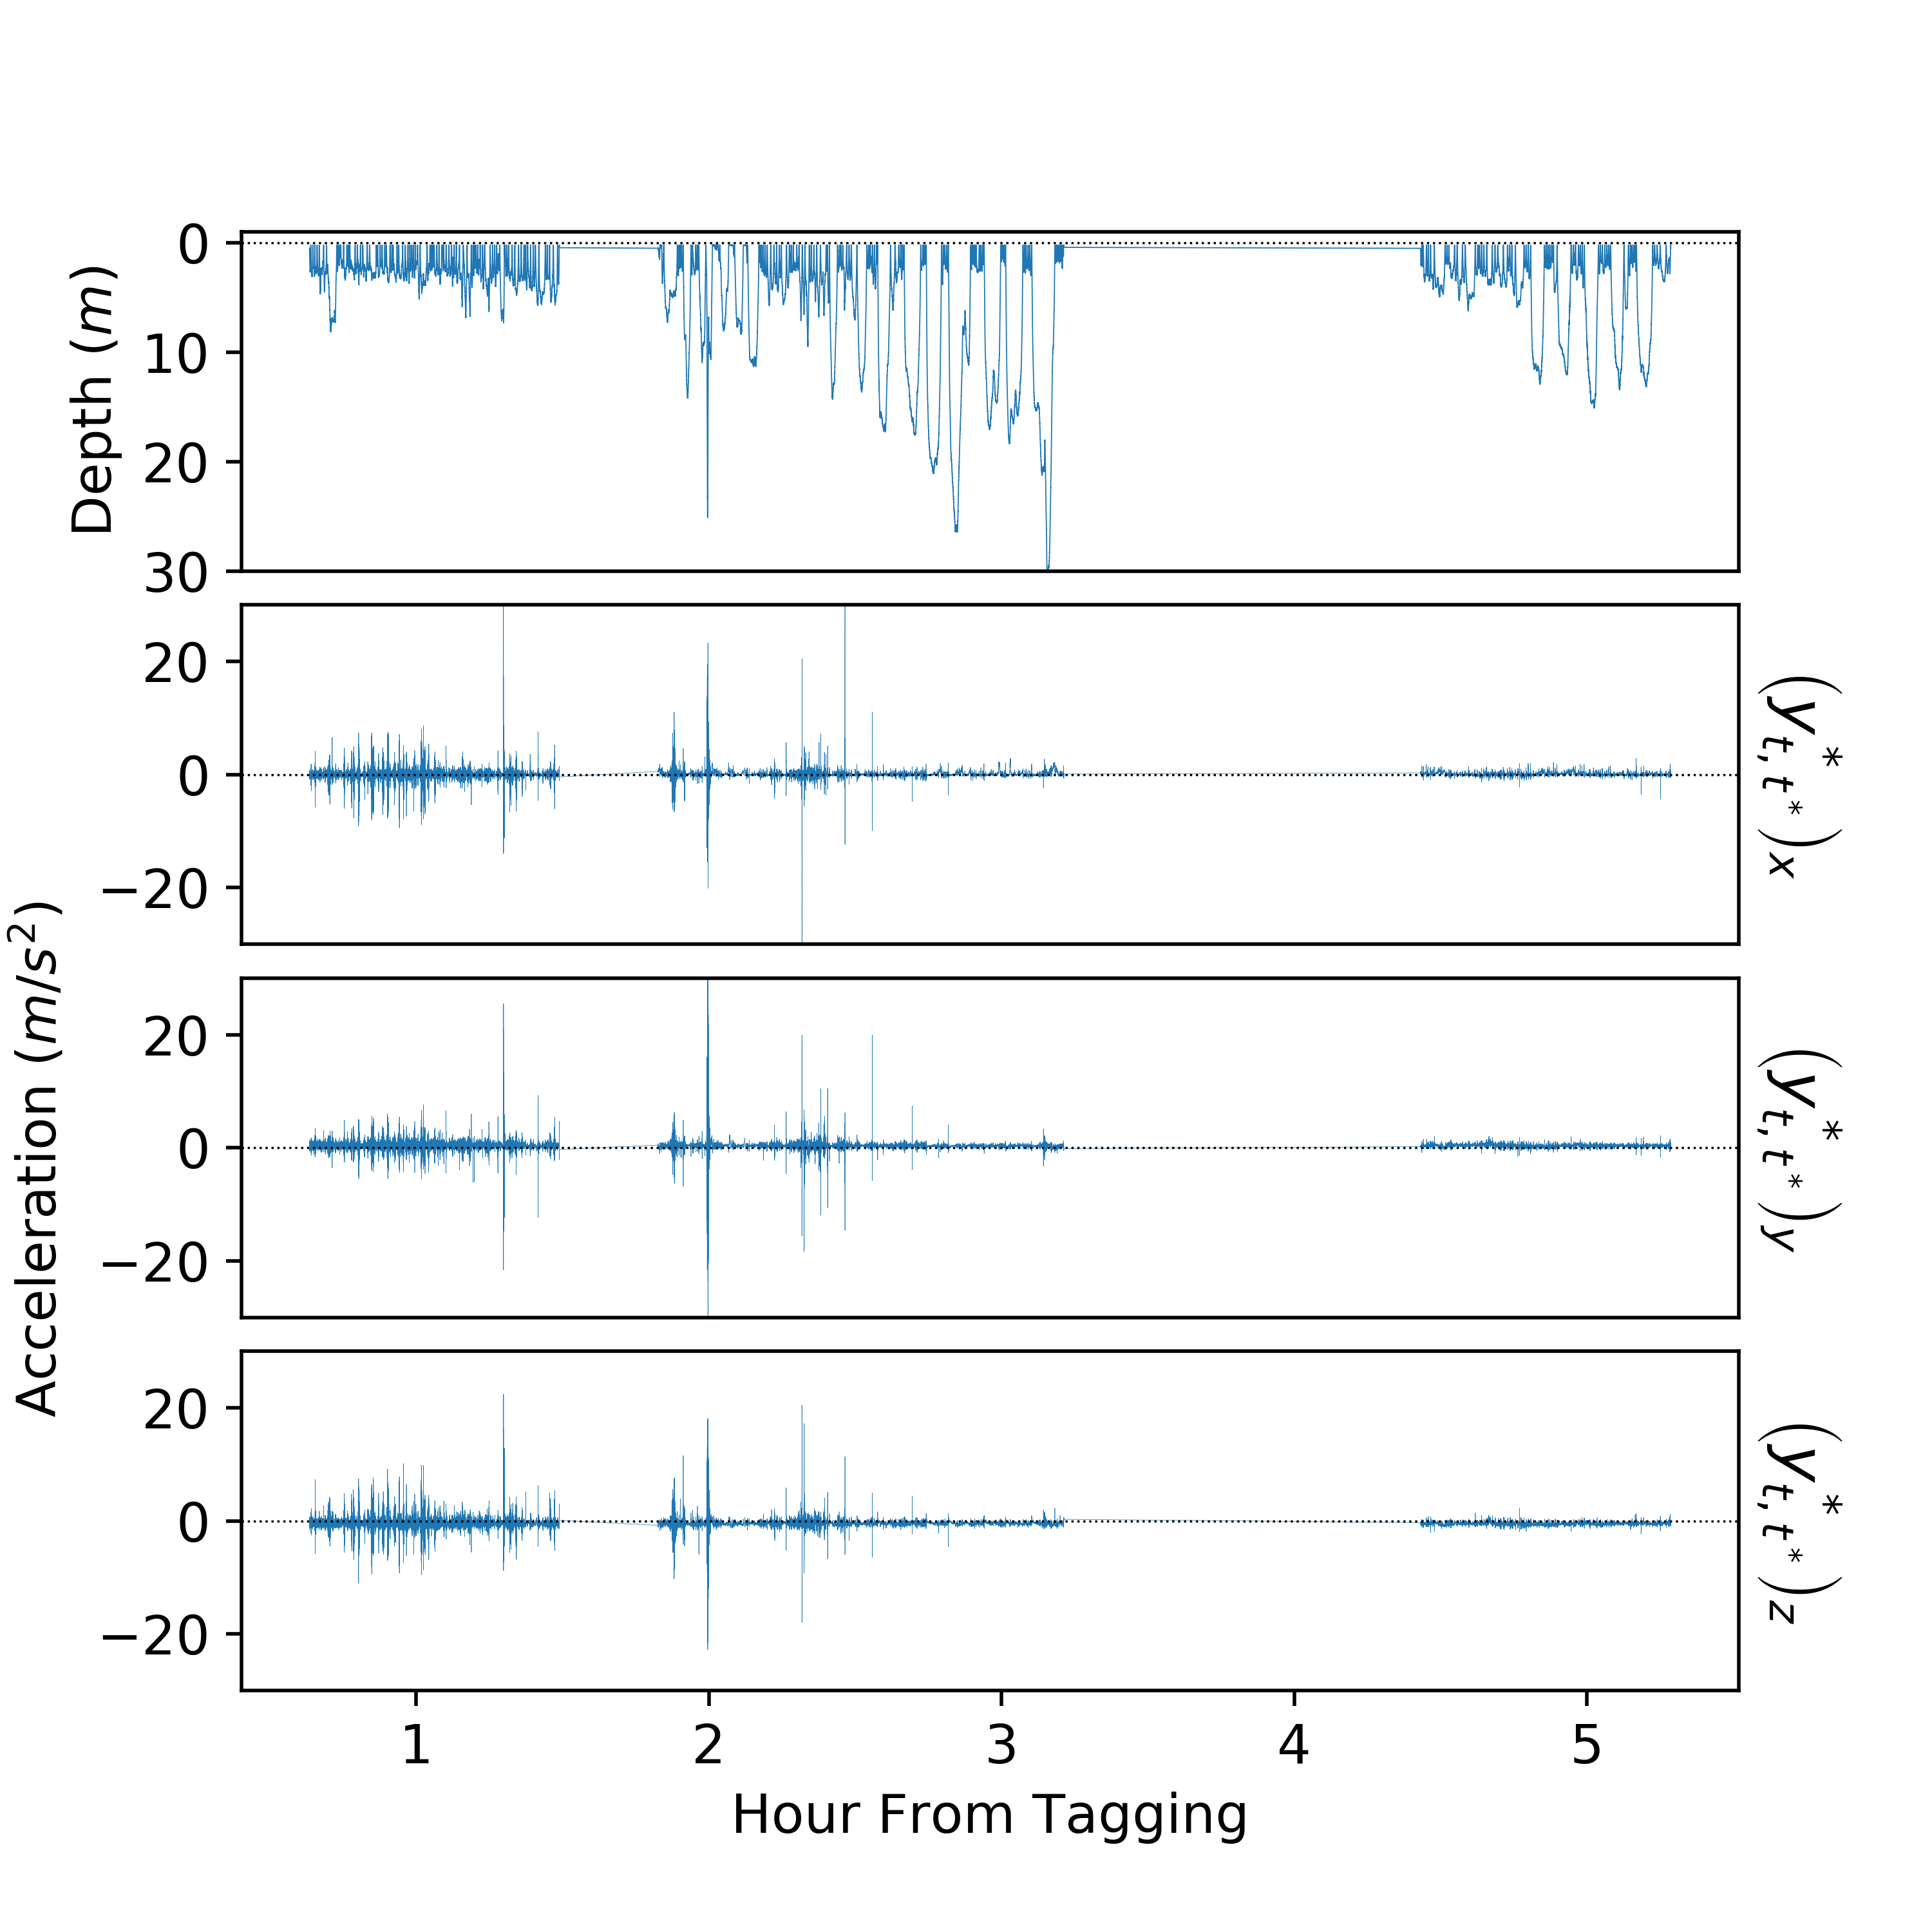
\includegraphics[width=5.5in]{../Plots/raw_data.png}
	\caption{Dive depth (top panel) and acceleration (bottom three panels) as functions of time from a Northern resident killer whale.}
	\label{fig:data}
\end{figure}

\begin{figure}[ht]
	\centering
	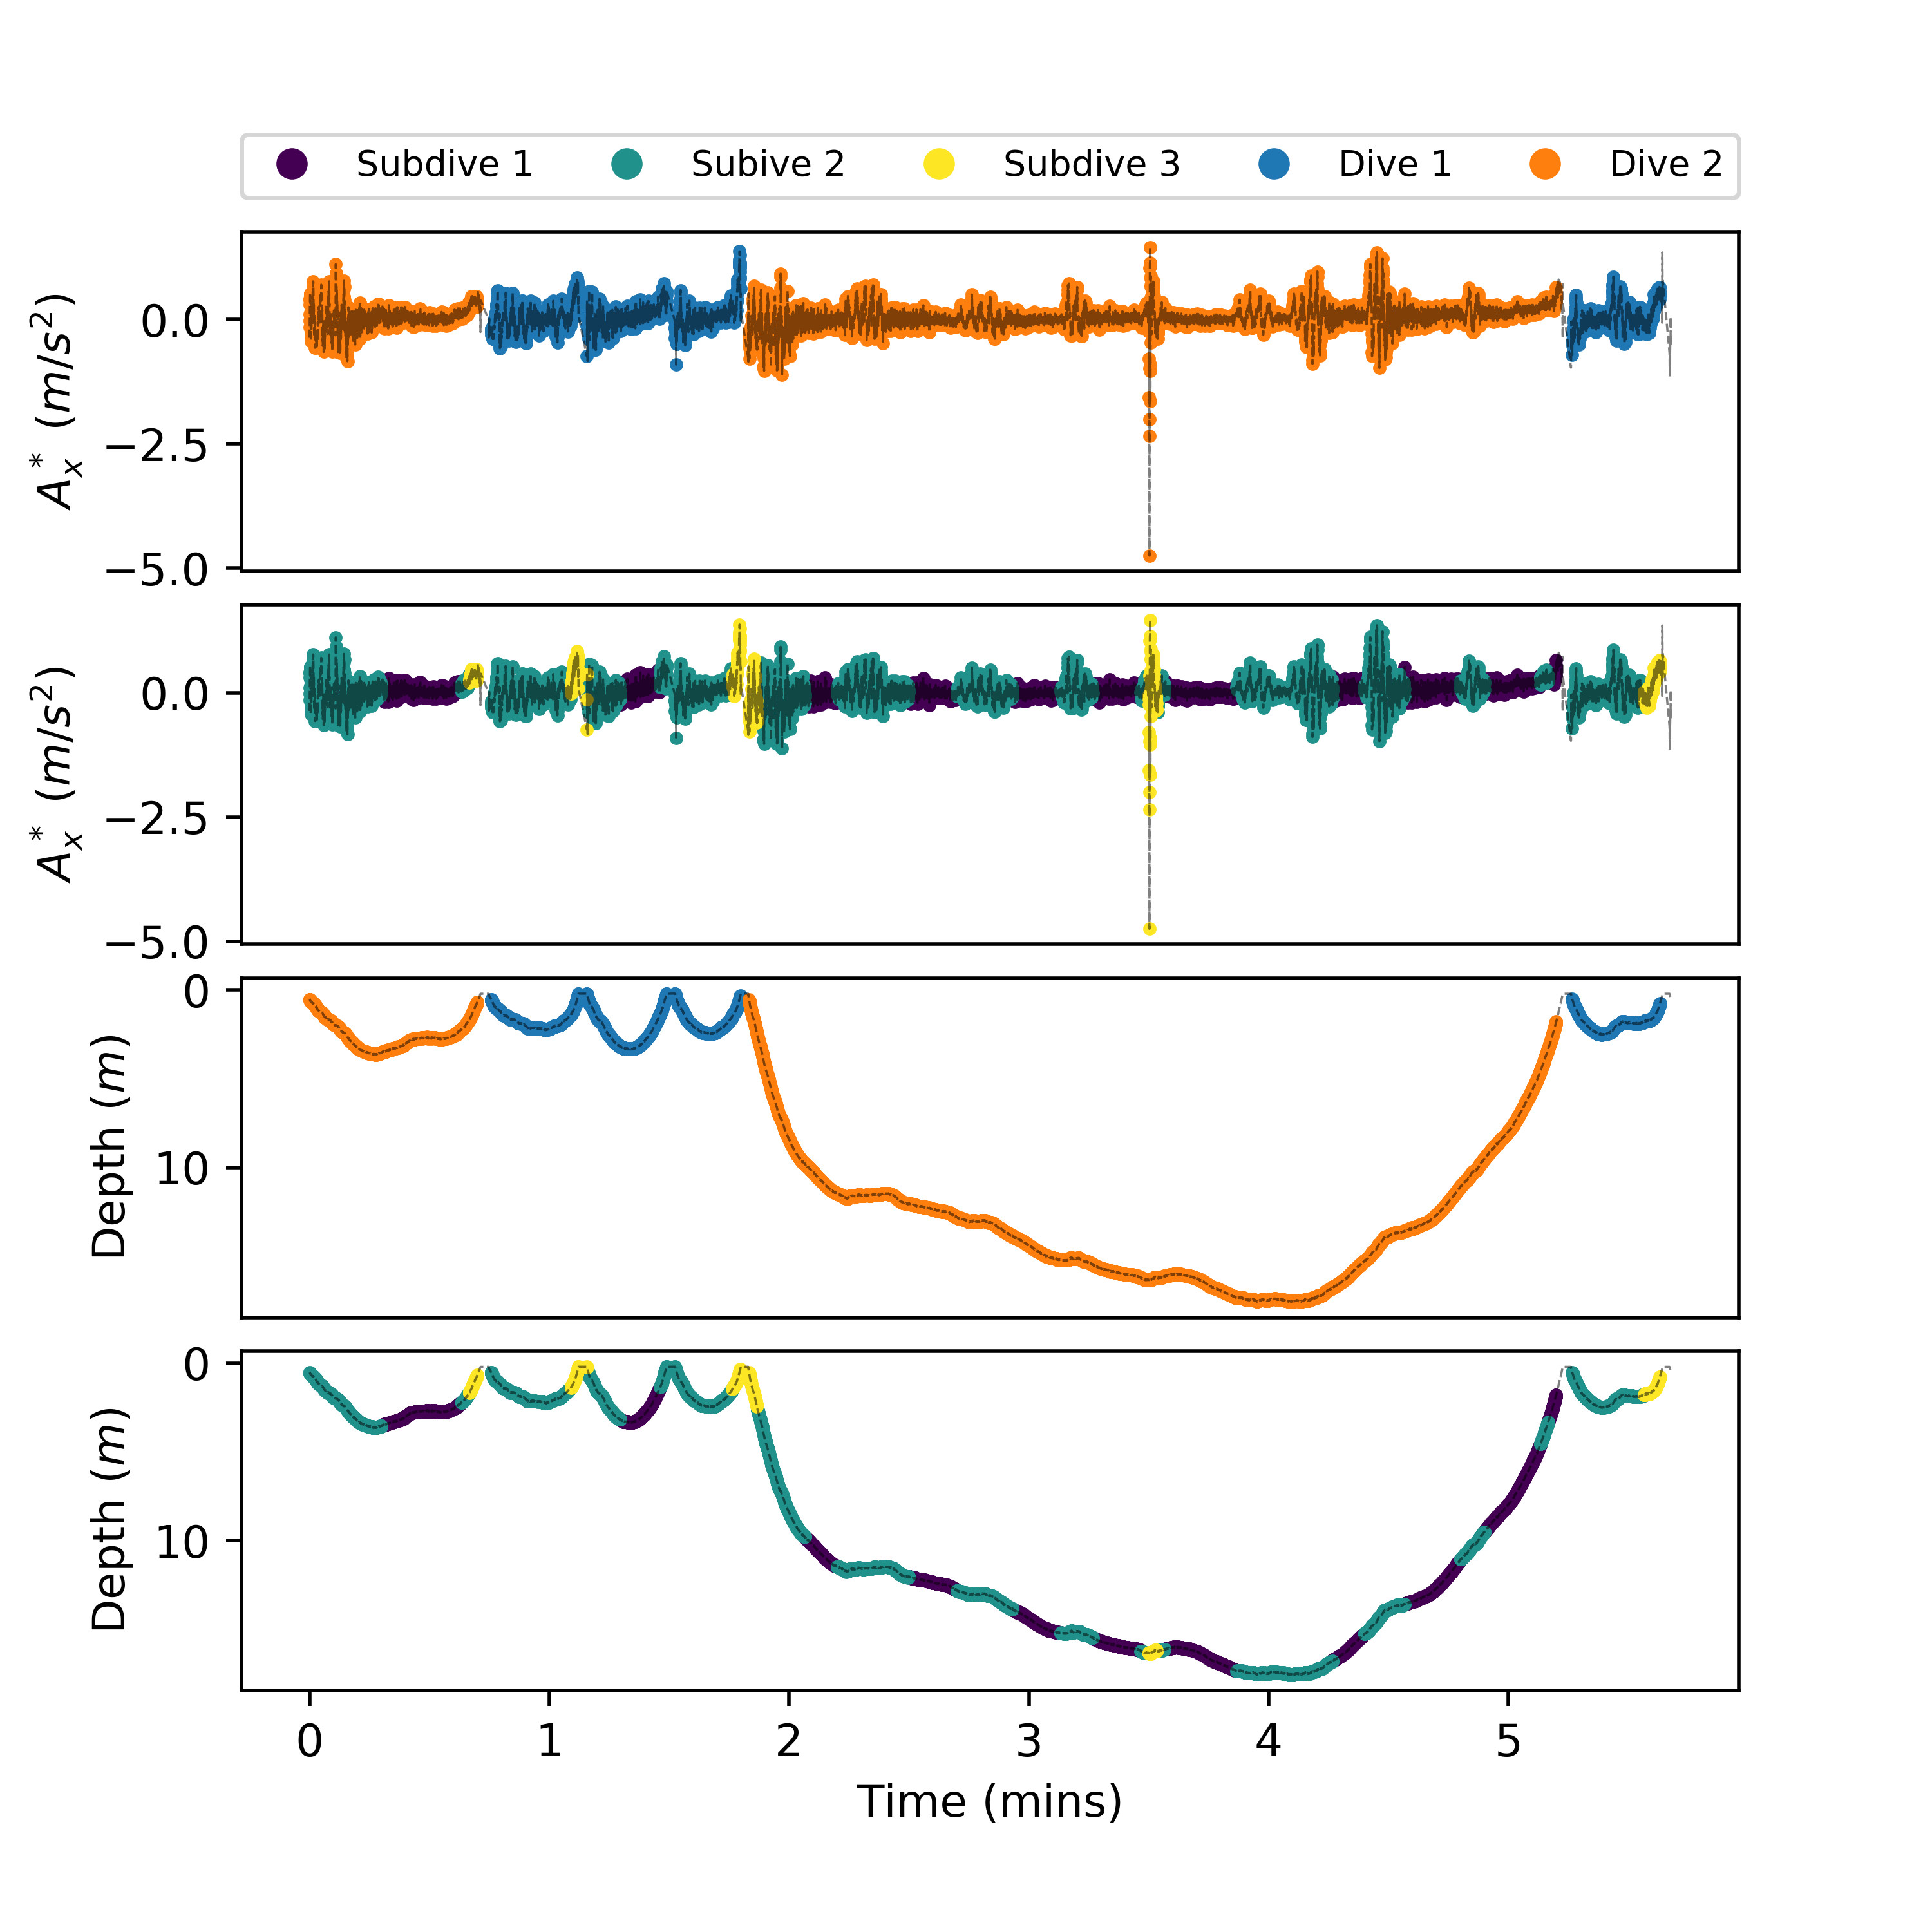
\includegraphics[width=5in]{../Plots/CarHHMM2_decoded_dives.png}
	\caption{The $x$-component of acceleration ($\Zone_x$) and dive profile of a Northern resident killer whale. The line colour of the first and third panels correspond to the estimated dive types while the line colour of the second and fourth panels show the estimated subdive states. Both the dive types and subdive states are estimated by fitting the CarHHMM-DFT to the data.}
	\label{fig:labeled_dives}
\end{figure}

%%% model definitions %%%

\begin{figure}[ht]
    \begin{subfigure}{\textwidth}
      \centering
      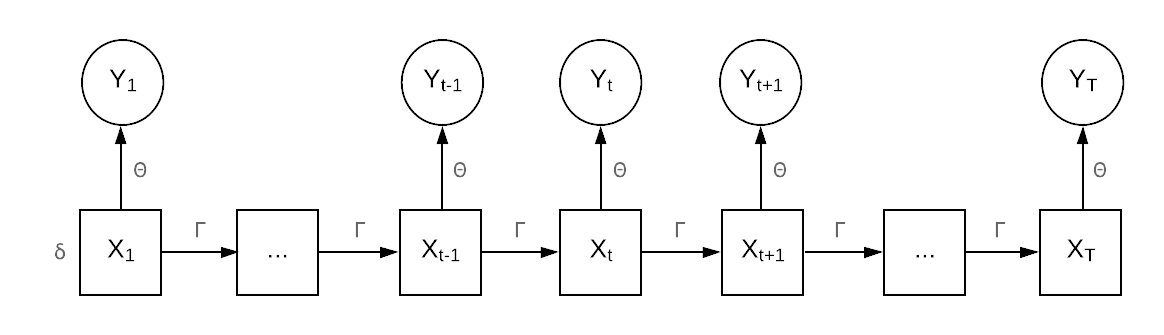
\includegraphics[width=4in]{../Plots/HMM.png}  
      \caption{Hidden Markov Model (\textbf{HMM})}
      \label{fig:HMM}
    \end{subfigure}
    %
    \newline
    %
    \begin{subfigure}{\textwidth}
      \centering
      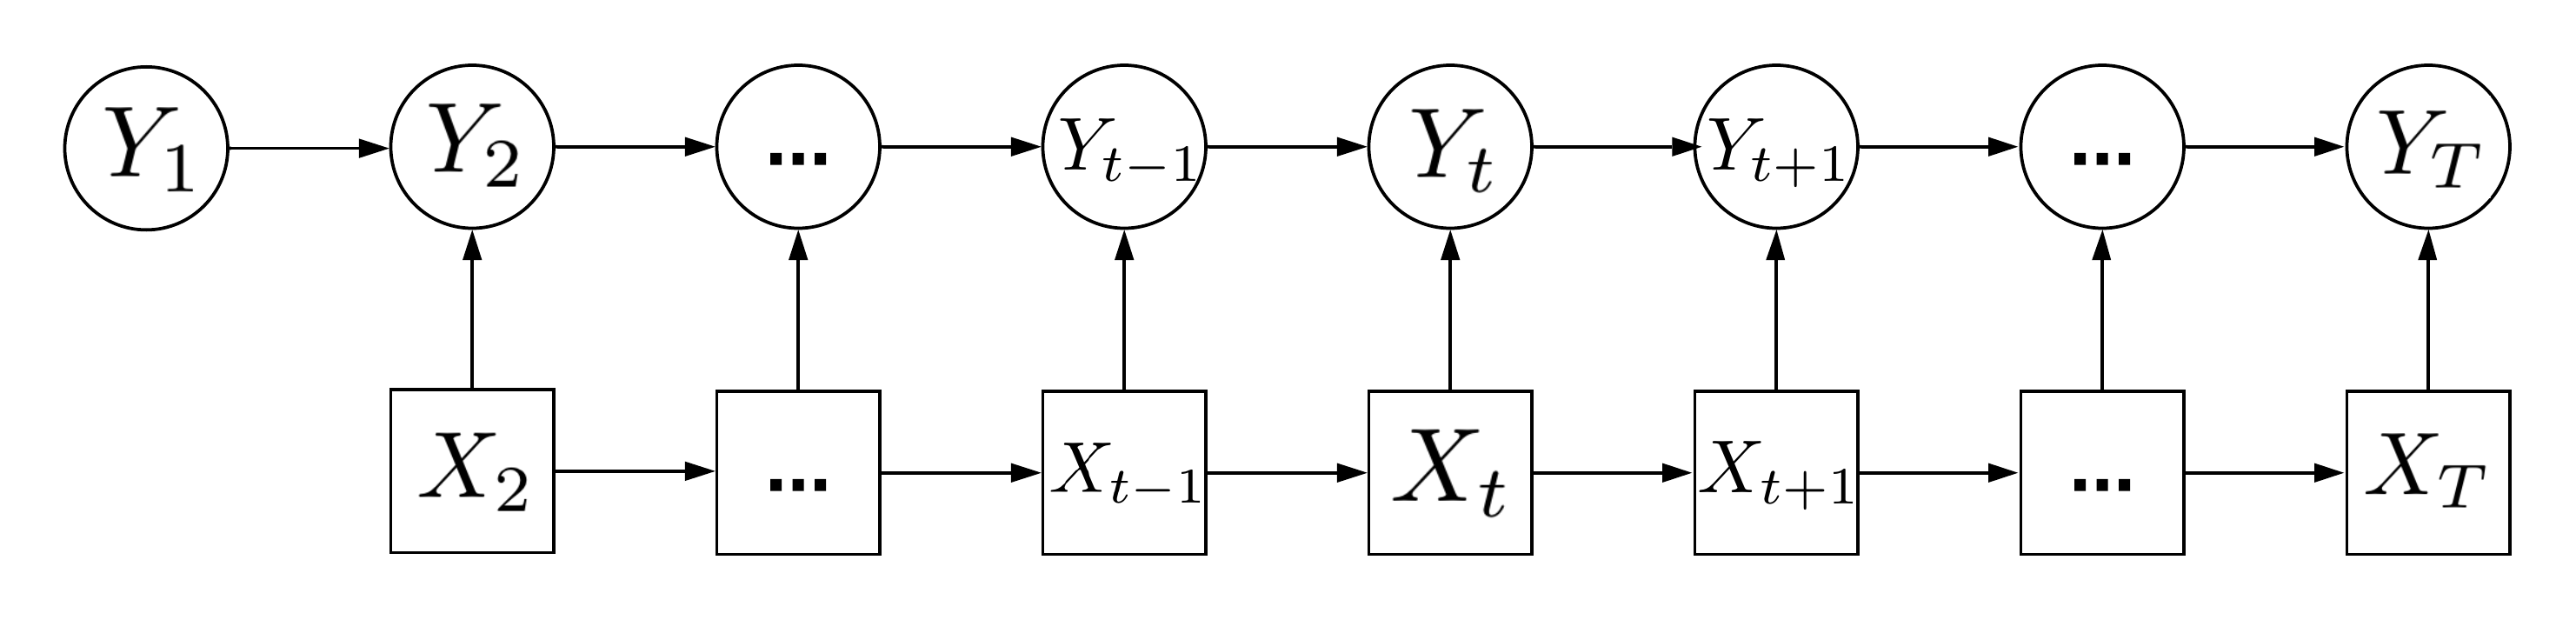
\includegraphics[width=4in]{../Plots/CarHMM.png}  
      \caption{Conditionally Auto-regressive HMM (\textbf{CarHMM})}
      \label{fig:CarHMM}
    \end{subfigure}
    %
    \newline
    %
    \begin{subfigure}{\textwidth}
      \centering
      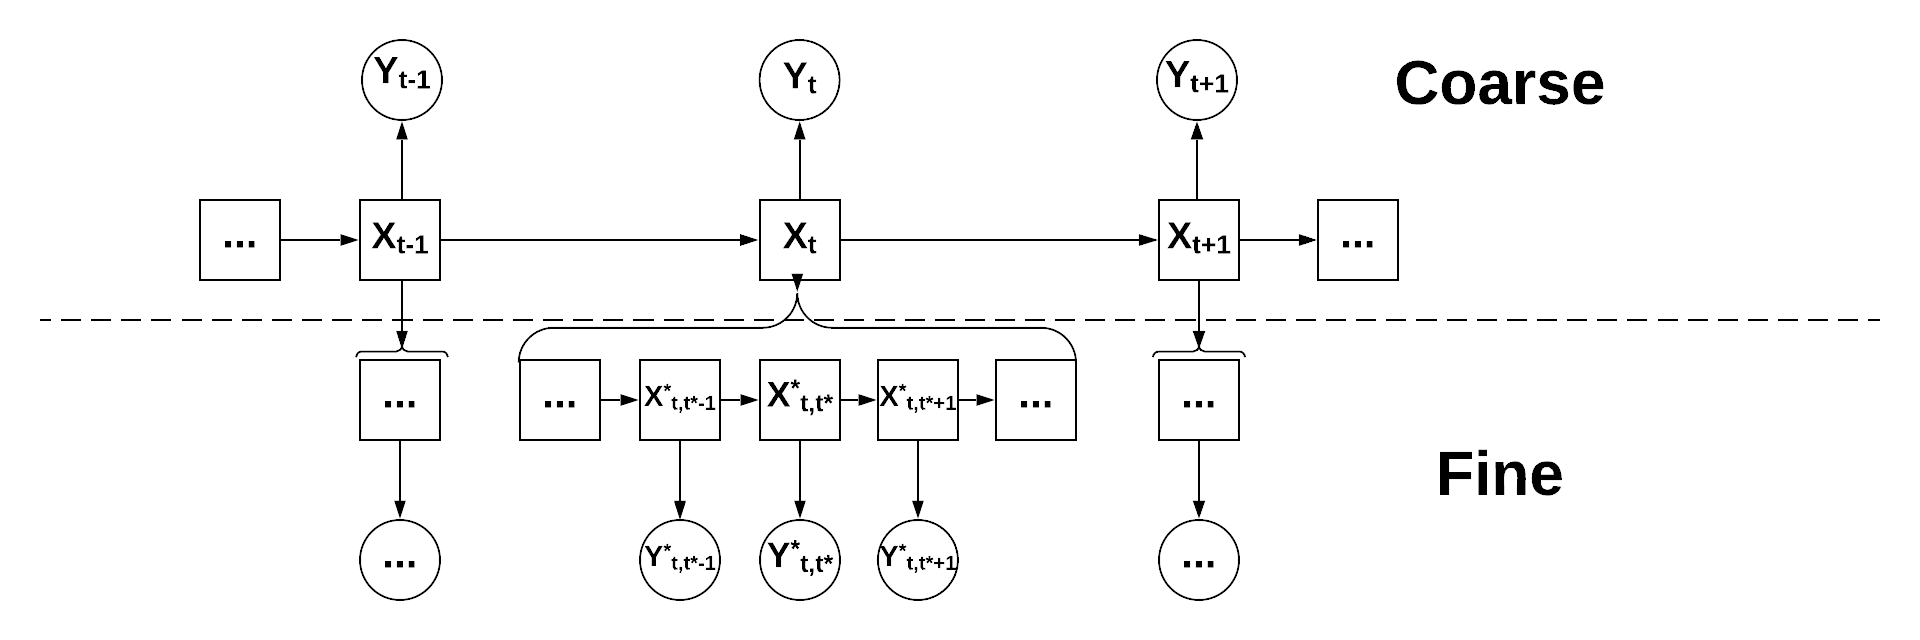
\includegraphics[width=4in]{../Plots/HHMM.png}  
      \caption{Hierarchical HMM (\textbf{HHMM})}
      \label{fig:HHMM}
    \end{subfigure}
    %
    \newline
    %
    \begin{subfigure}{\textwidth}
      \centering
      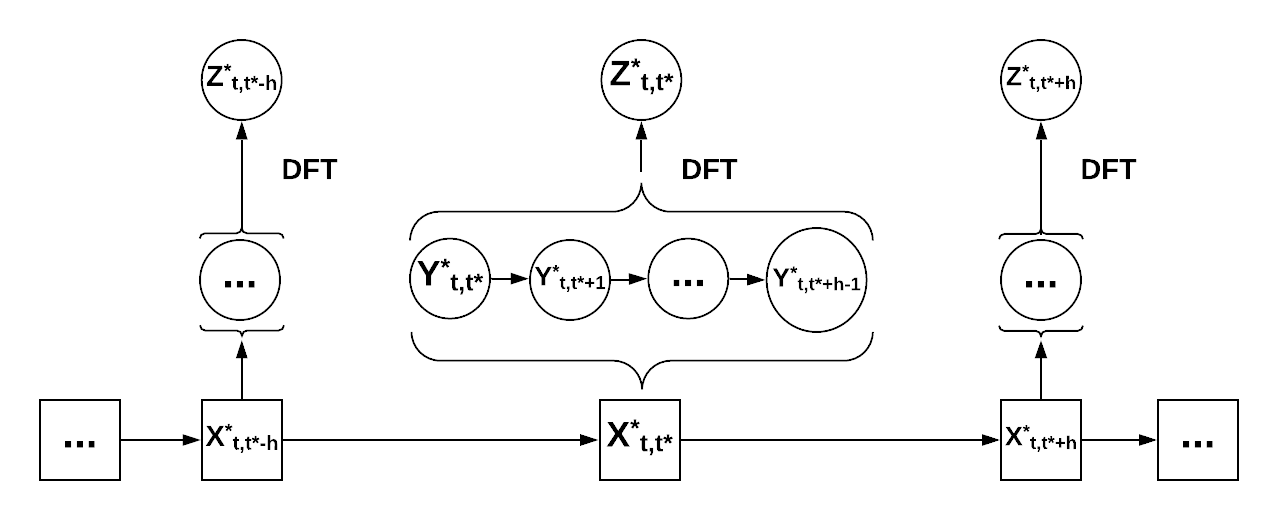
\includegraphics[width=4in]{../Plots/HMM-DFT.png}  
      \caption{HMM with Discrete Fourier Transform (\textbf{HMM-DFT})}
      \label{fig:HMM-DFT}
    \end{subfigure}
    \caption{Dependence structures of several different types of HMM-based models.}
    \label{fig:models}
\end{figure}

%%% Case Study %%%

\begin{figure}[ht]
	\centering
	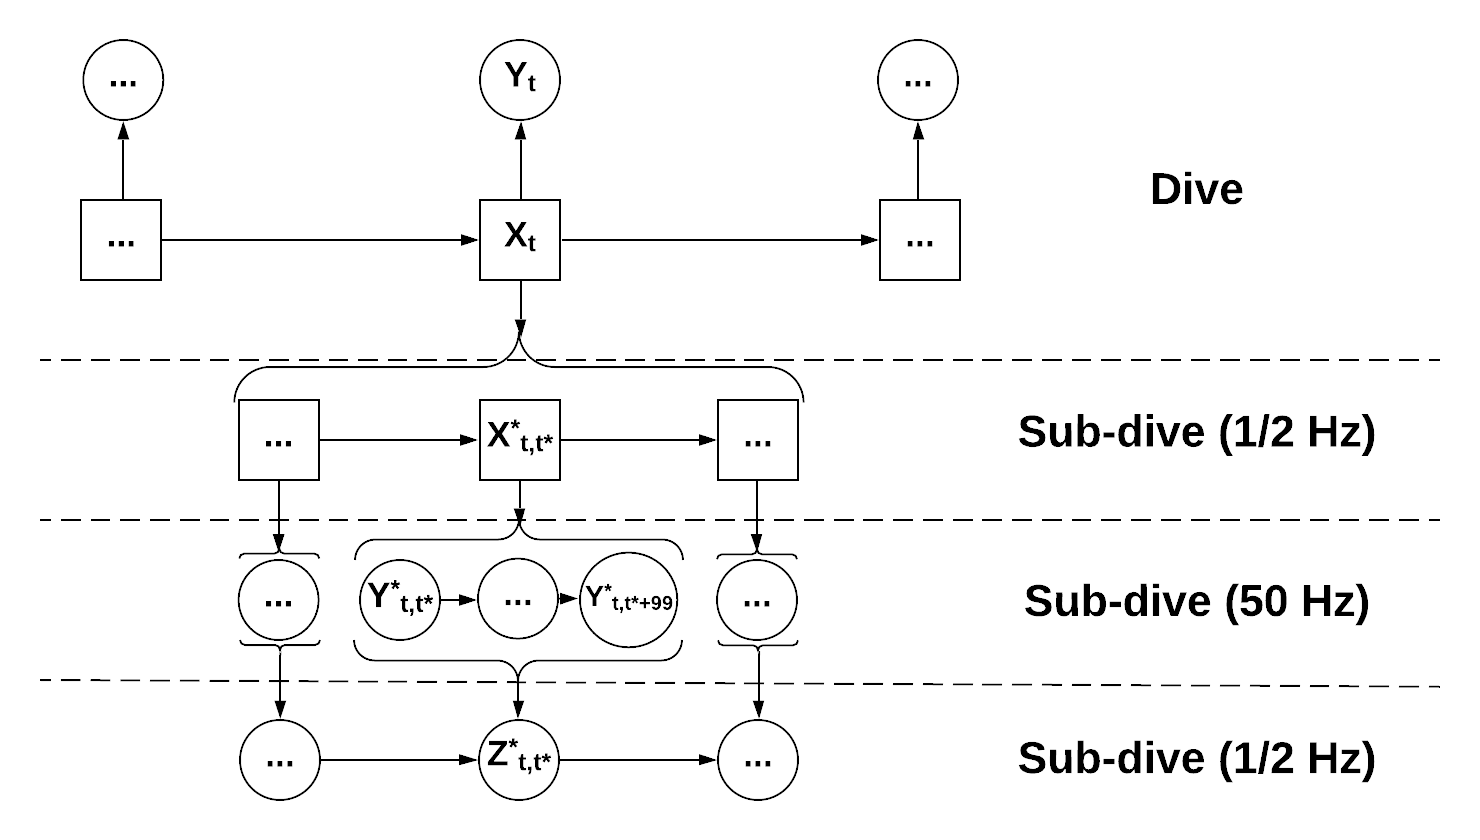
\includegraphics[width=5in]{../Plots/CarHHMM-DFT.png}
	\caption{Graphical representation the model used in the simulation and case study, the \textbf{CarHHMM-DFT}.}
	\label{fig:CarHHMM-DFT}
\end{figure}

\begin{figure}[ht]
	\centering
	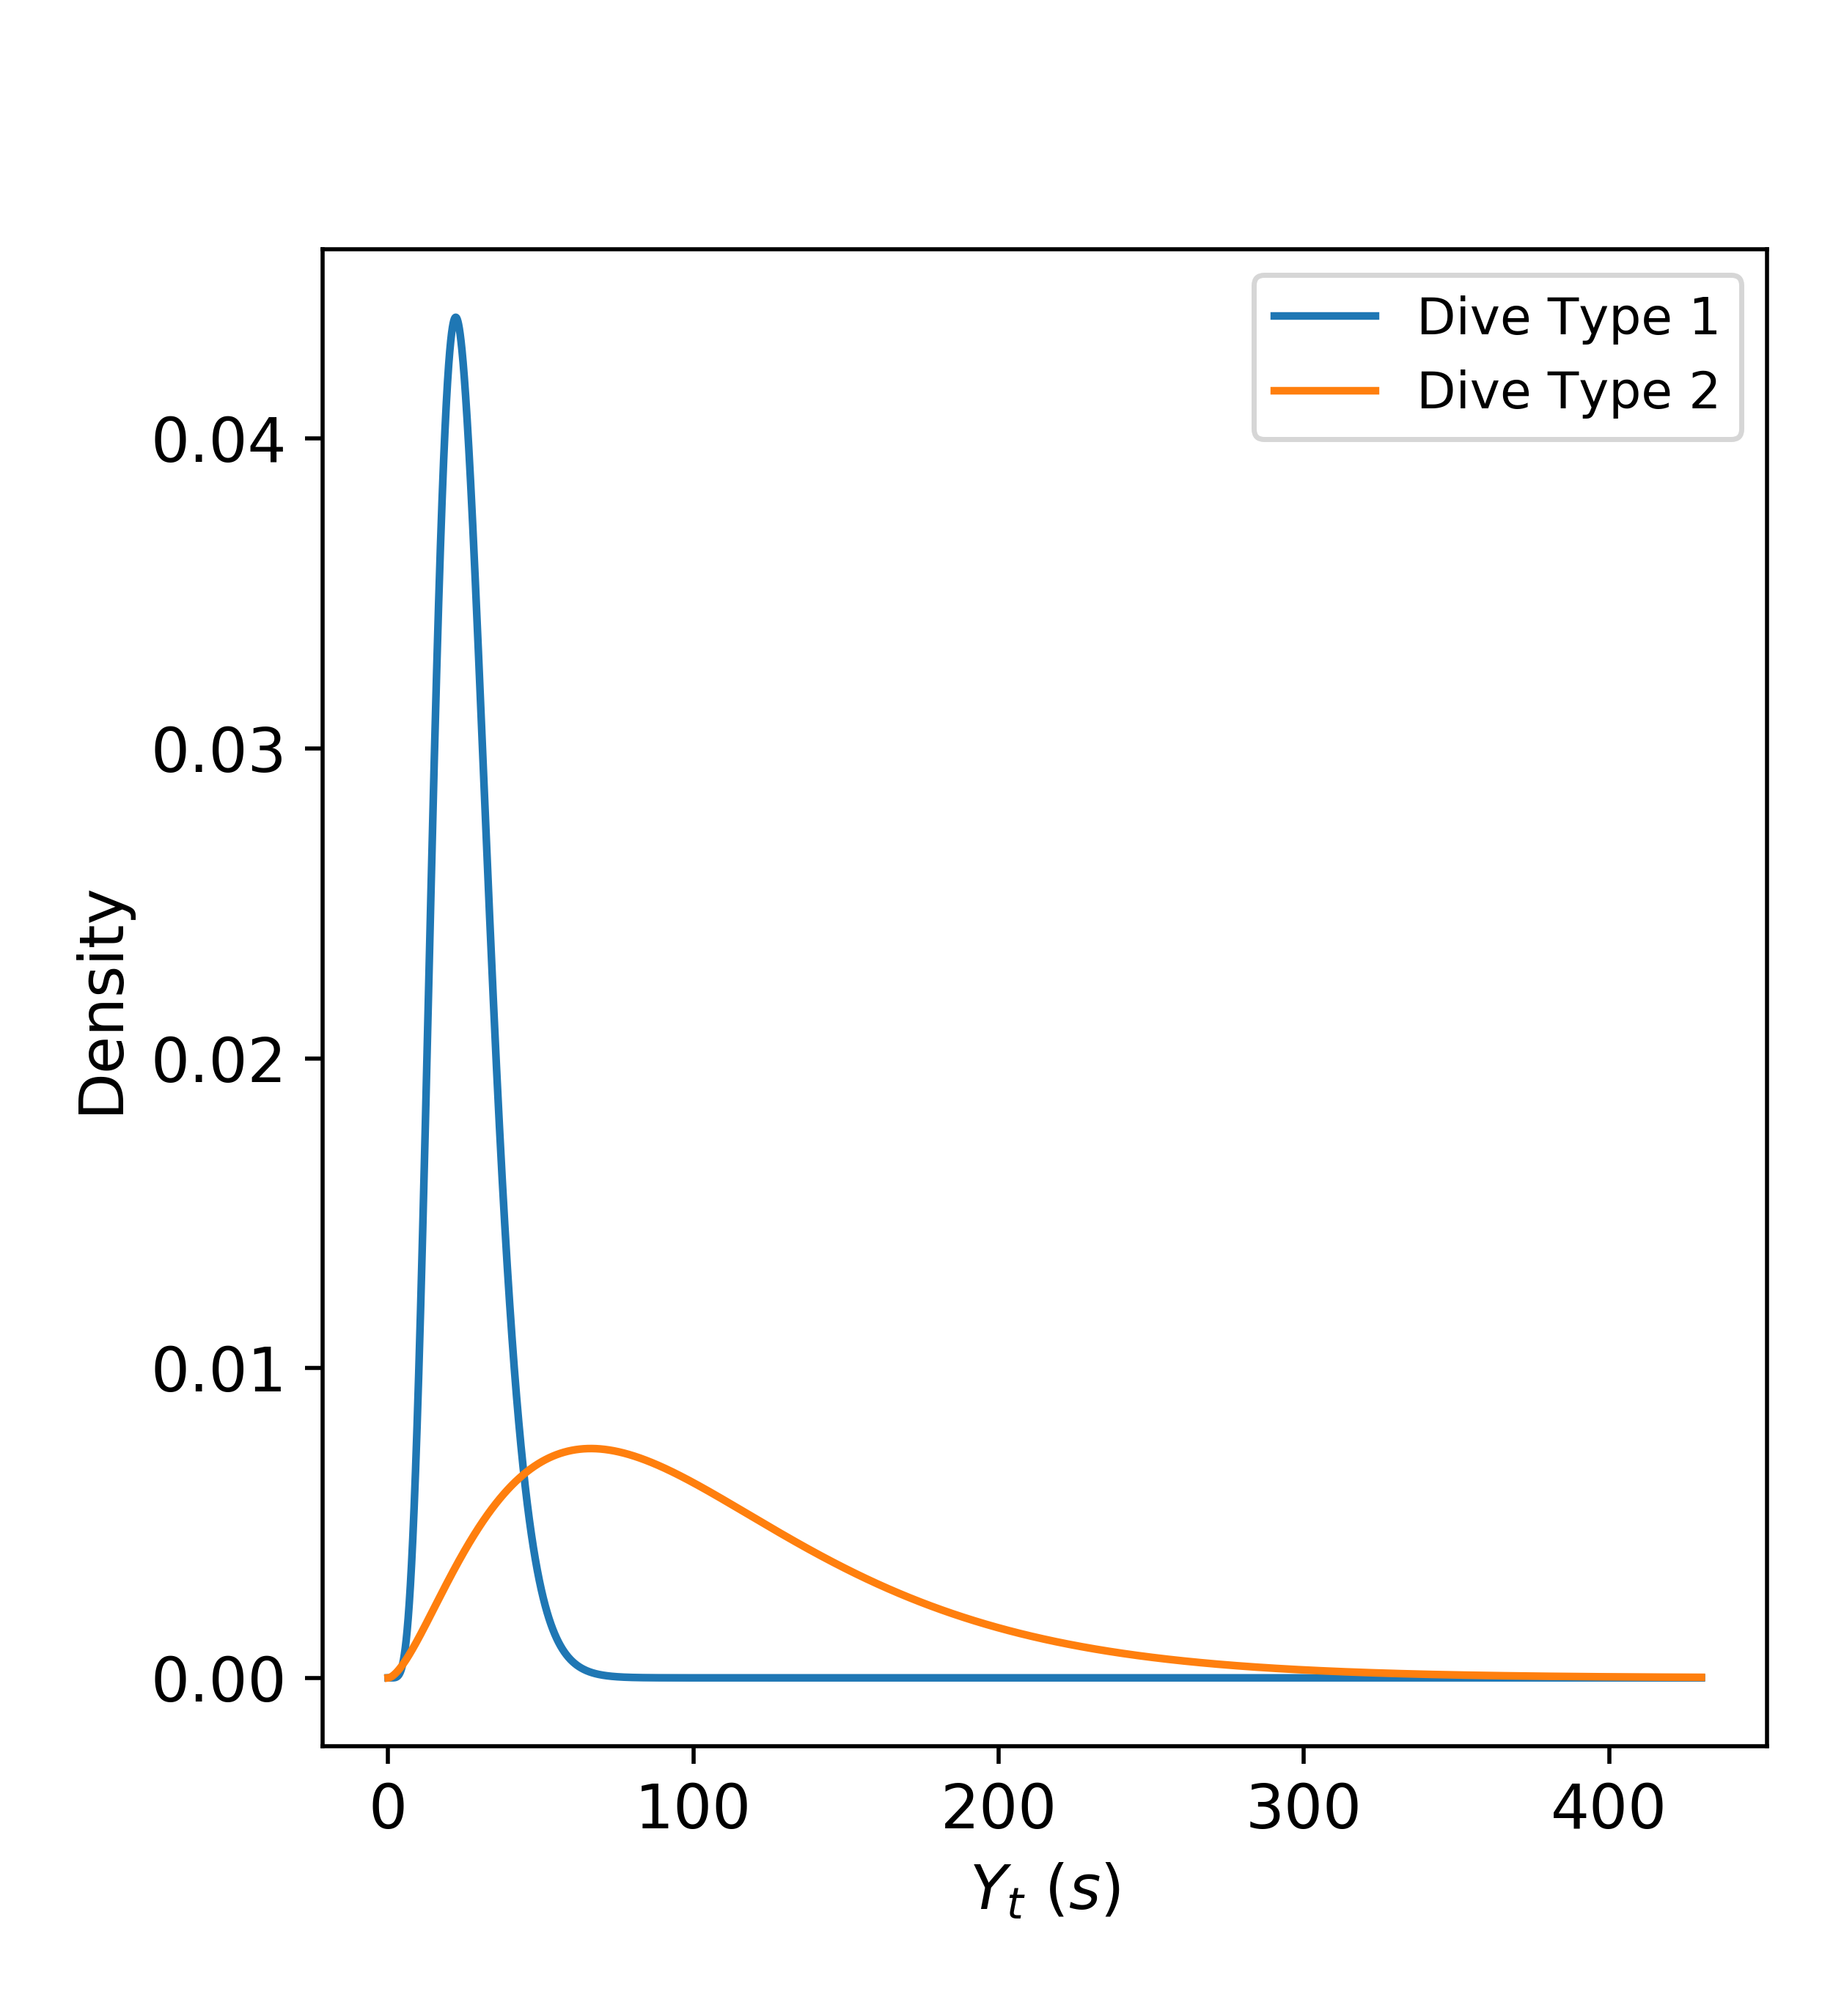
\includegraphics[width=5in]{../Plots/CarHHMM2-coarse-emissions.png}
	\caption{Estimated probability densities of dive duration ($Y$) corresponding to dive type 1 (short dives) and dive type 2 (longer dives). These are Gamma distributions and are fit using the CarHHMM-DFT and the killer whale case study data.}
	\label{fig:coarse_emis}
\end{figure}

\begin{figure}[ht]
	\centering
	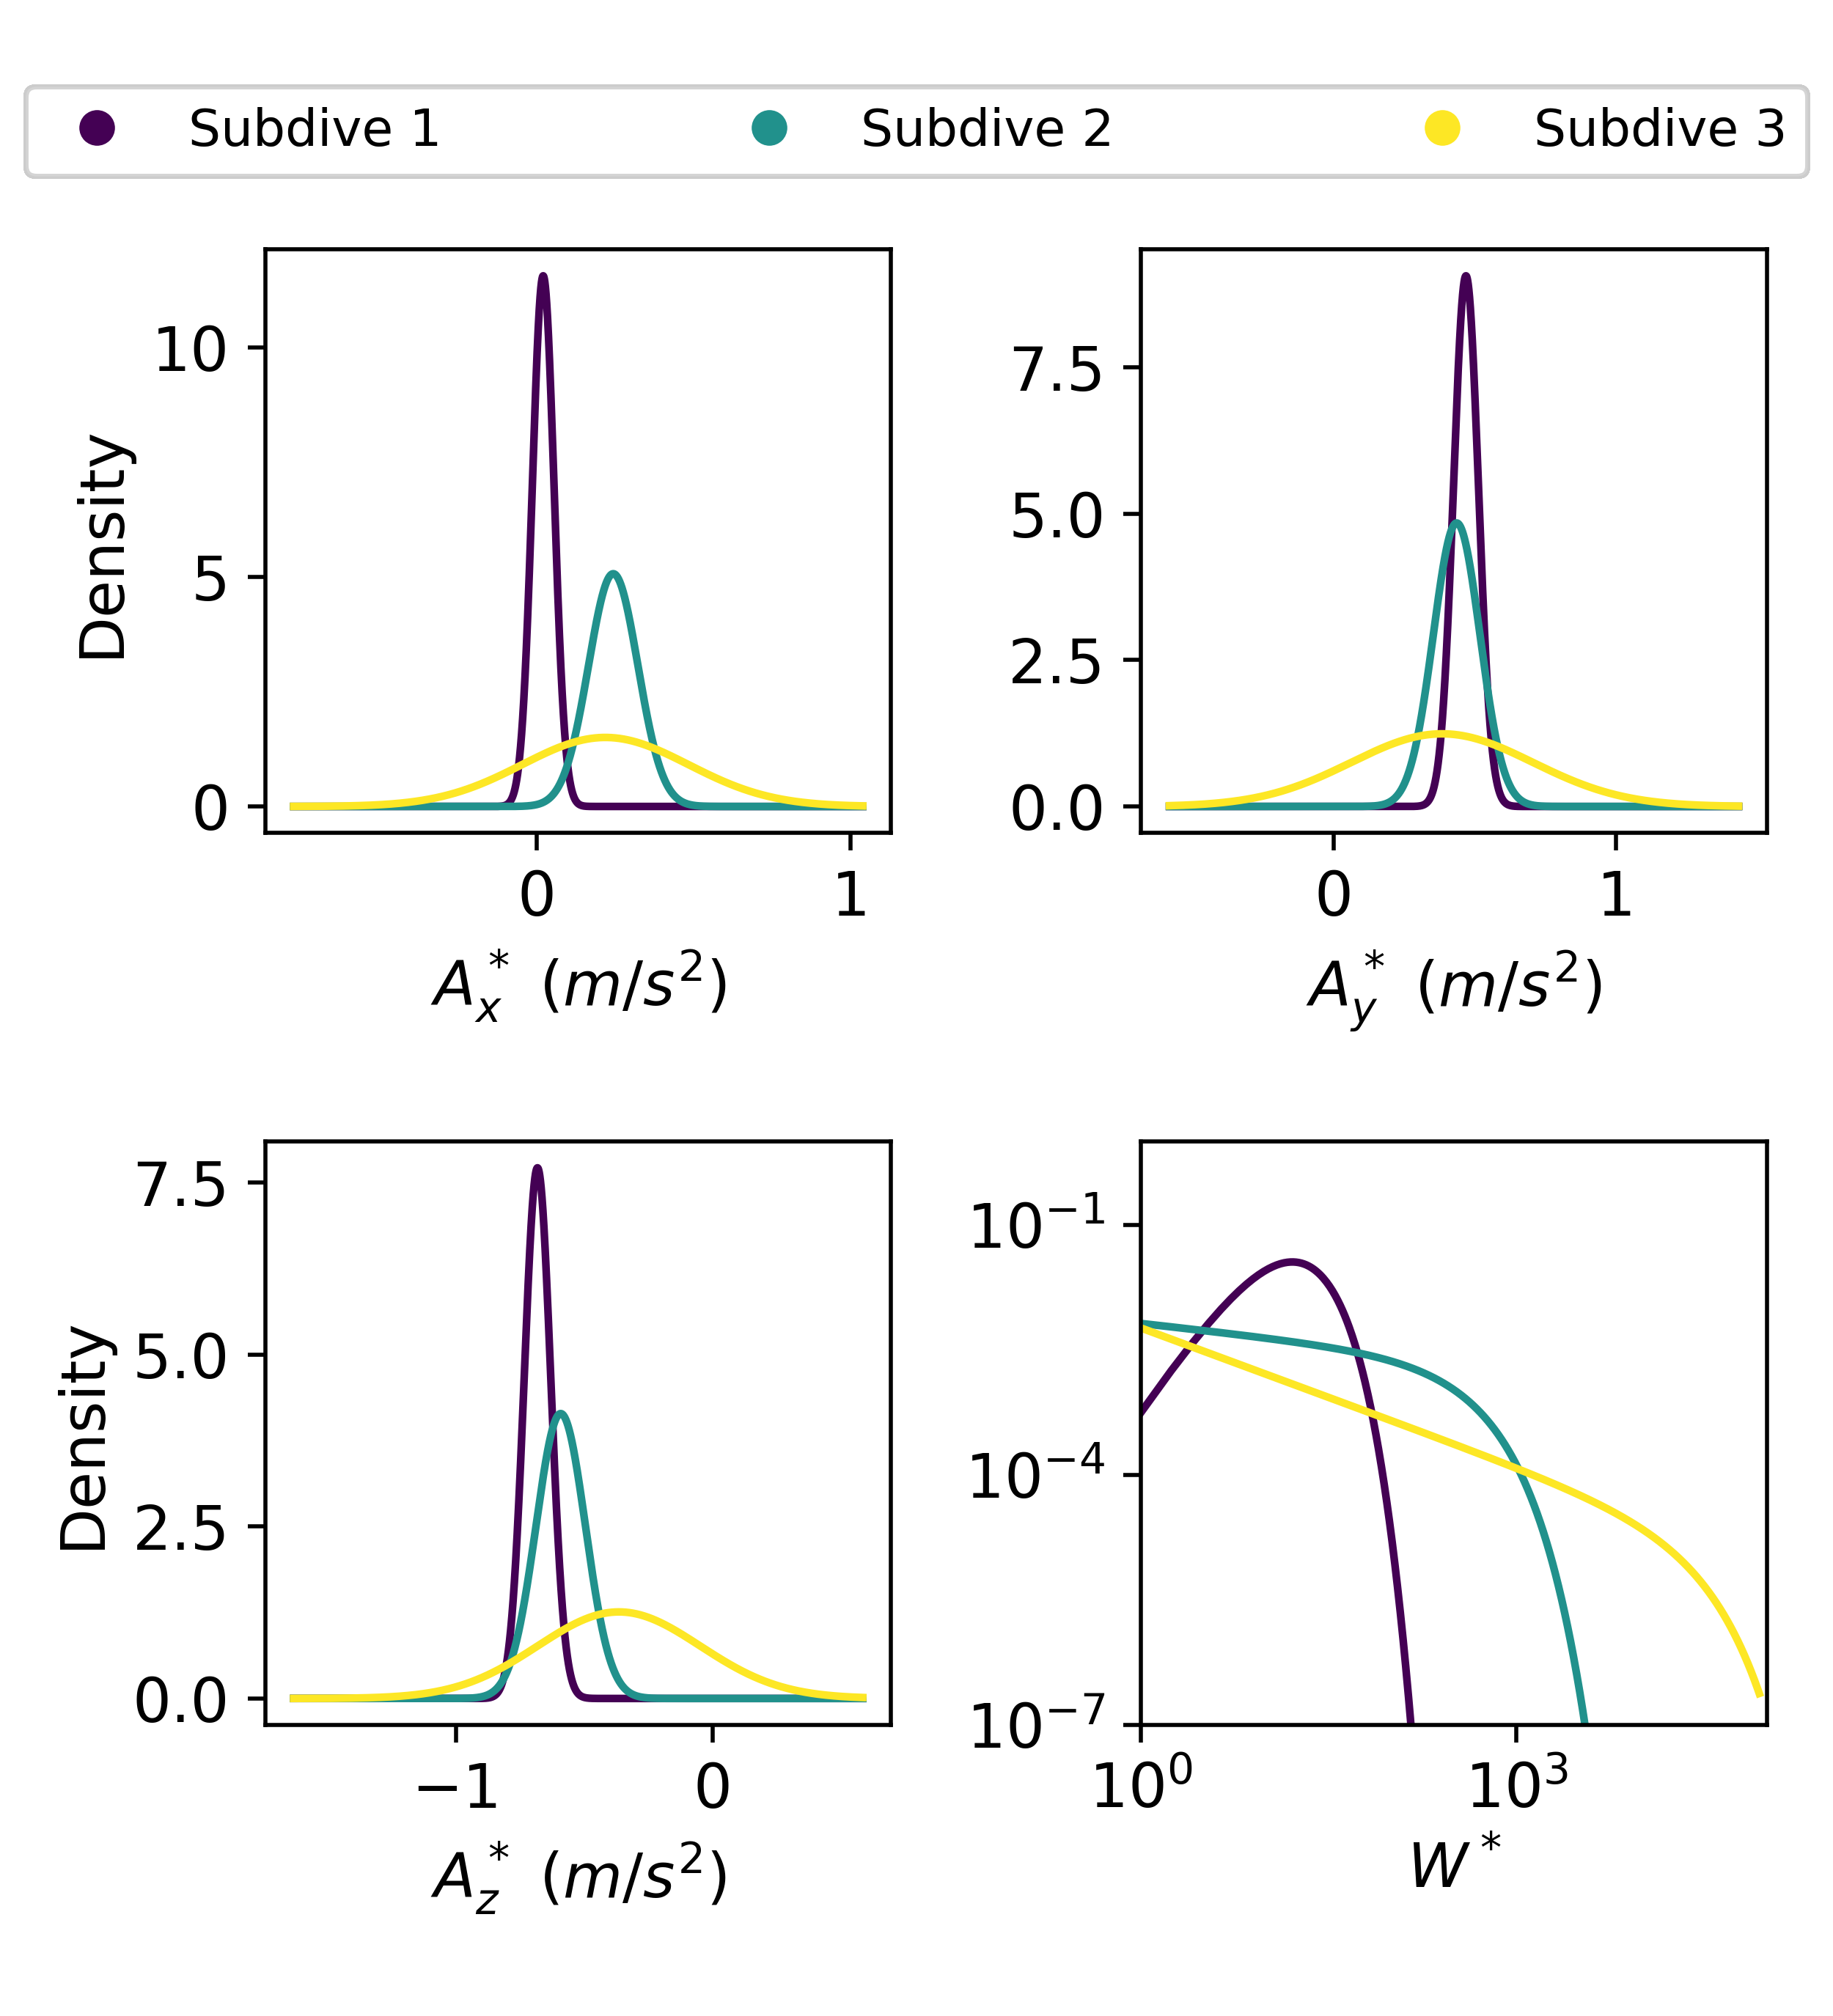
\includegraphics[width=5in]{../Plots/CarHHMM2-fine-emissions.png}
	\caption{Estimated probability densities acceleration ($\Zone$) and wiggliness ($\Ztwo$) corresponding to subdive states 1, 2 and 3. Densities corresponding to acceleration ($\Zone$) are Normal and do not take auto-correlation into account, meaning that the true long-run variation is larger than what is pictured here (see Table \ref{table:emis_dists_CarHHMM-DFT}). The estimated density of wiggliness ($\Ztwo$) is Gamma, and plotted on a log-log scale here for clarity.}
	\label{fig:fine_emis}
\end{figure}

\begin{figure}[ht]
    \begin{subfigure}{0.45\textwidth}
    	\centering
    	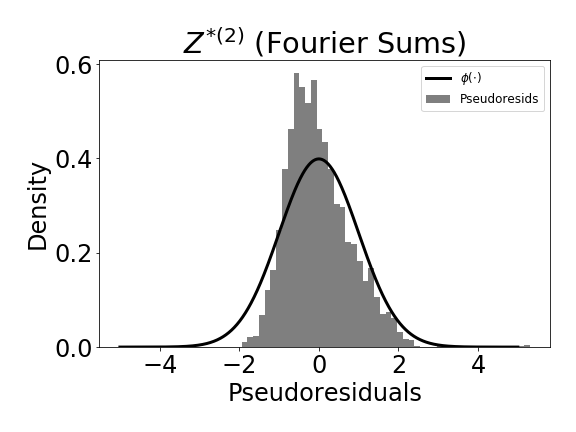
\includegraphics[width=2.25in]{../Plots/CarHHMM2_psedoresids_ahat.png}
    	\caption{Histogram of pseudoresiduals of $W^*$}
    	\label{fig:pseudoresids}
    \end{subfigure}
    \begin{subfigure}{0.45\textwidth}
    	\centering
    	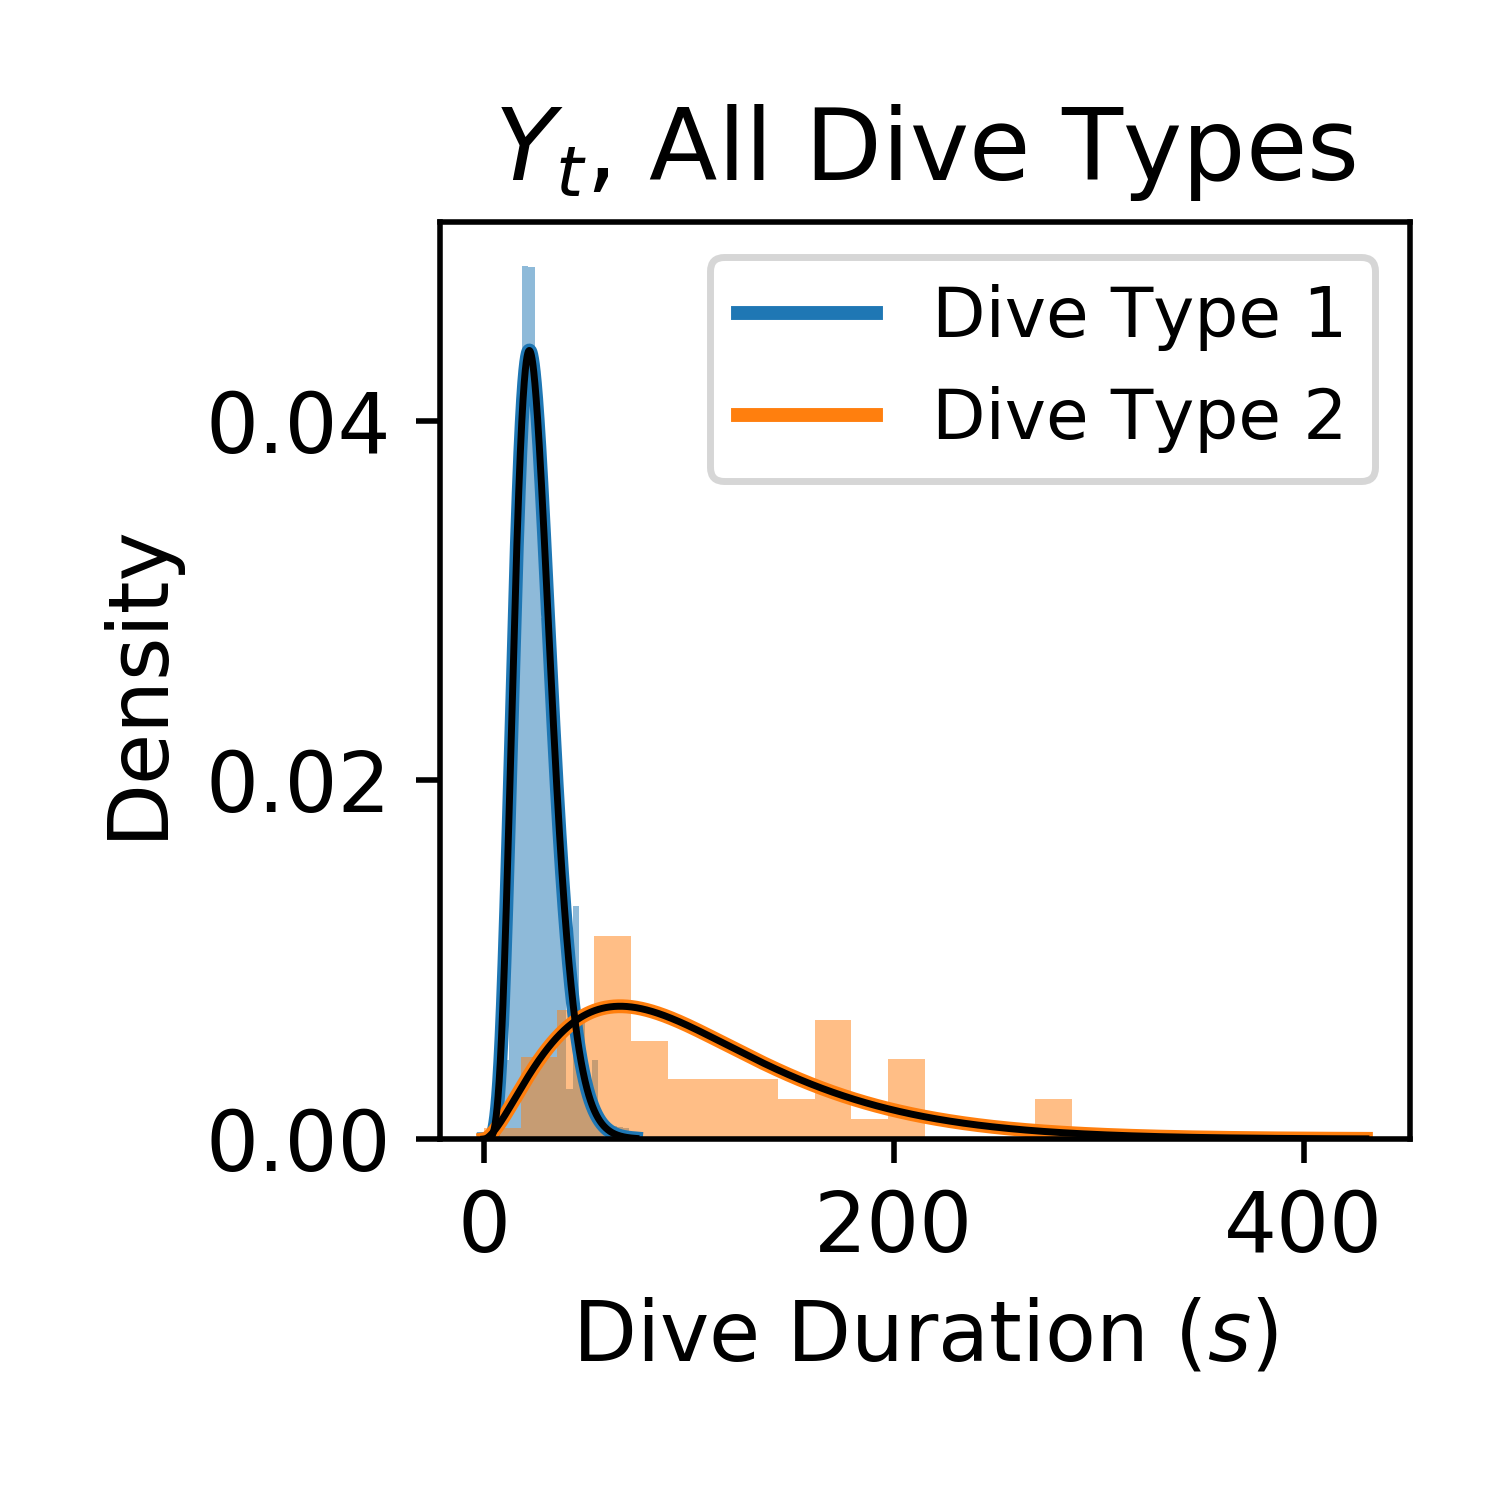
\includegraphics[width=2.25in]{../Plots/CarHHMM2_empirical_hist_dive_duration.png}
    	\caption{Empirical distribution of $Y$}
    	\label{fig:empirical_dist}
    \end{subfigure}
    \caption{Psuedoresiduals of wiggliness ($\Zone$, left) plotted over a standard normal density as well as a weighted empirical distribution of dive duration ($Y$, left) plotted over the fitted gamma distributions. Both plots are generated using the fitted CarHHMM-DFT and the Killer whale case study data. They severe as examples of model-checking tools for HMMs.}
    \label{fig:model_checking}
\end{figure}

%%% simulation study %%%

\begin{figure}[ht]
	\centering
	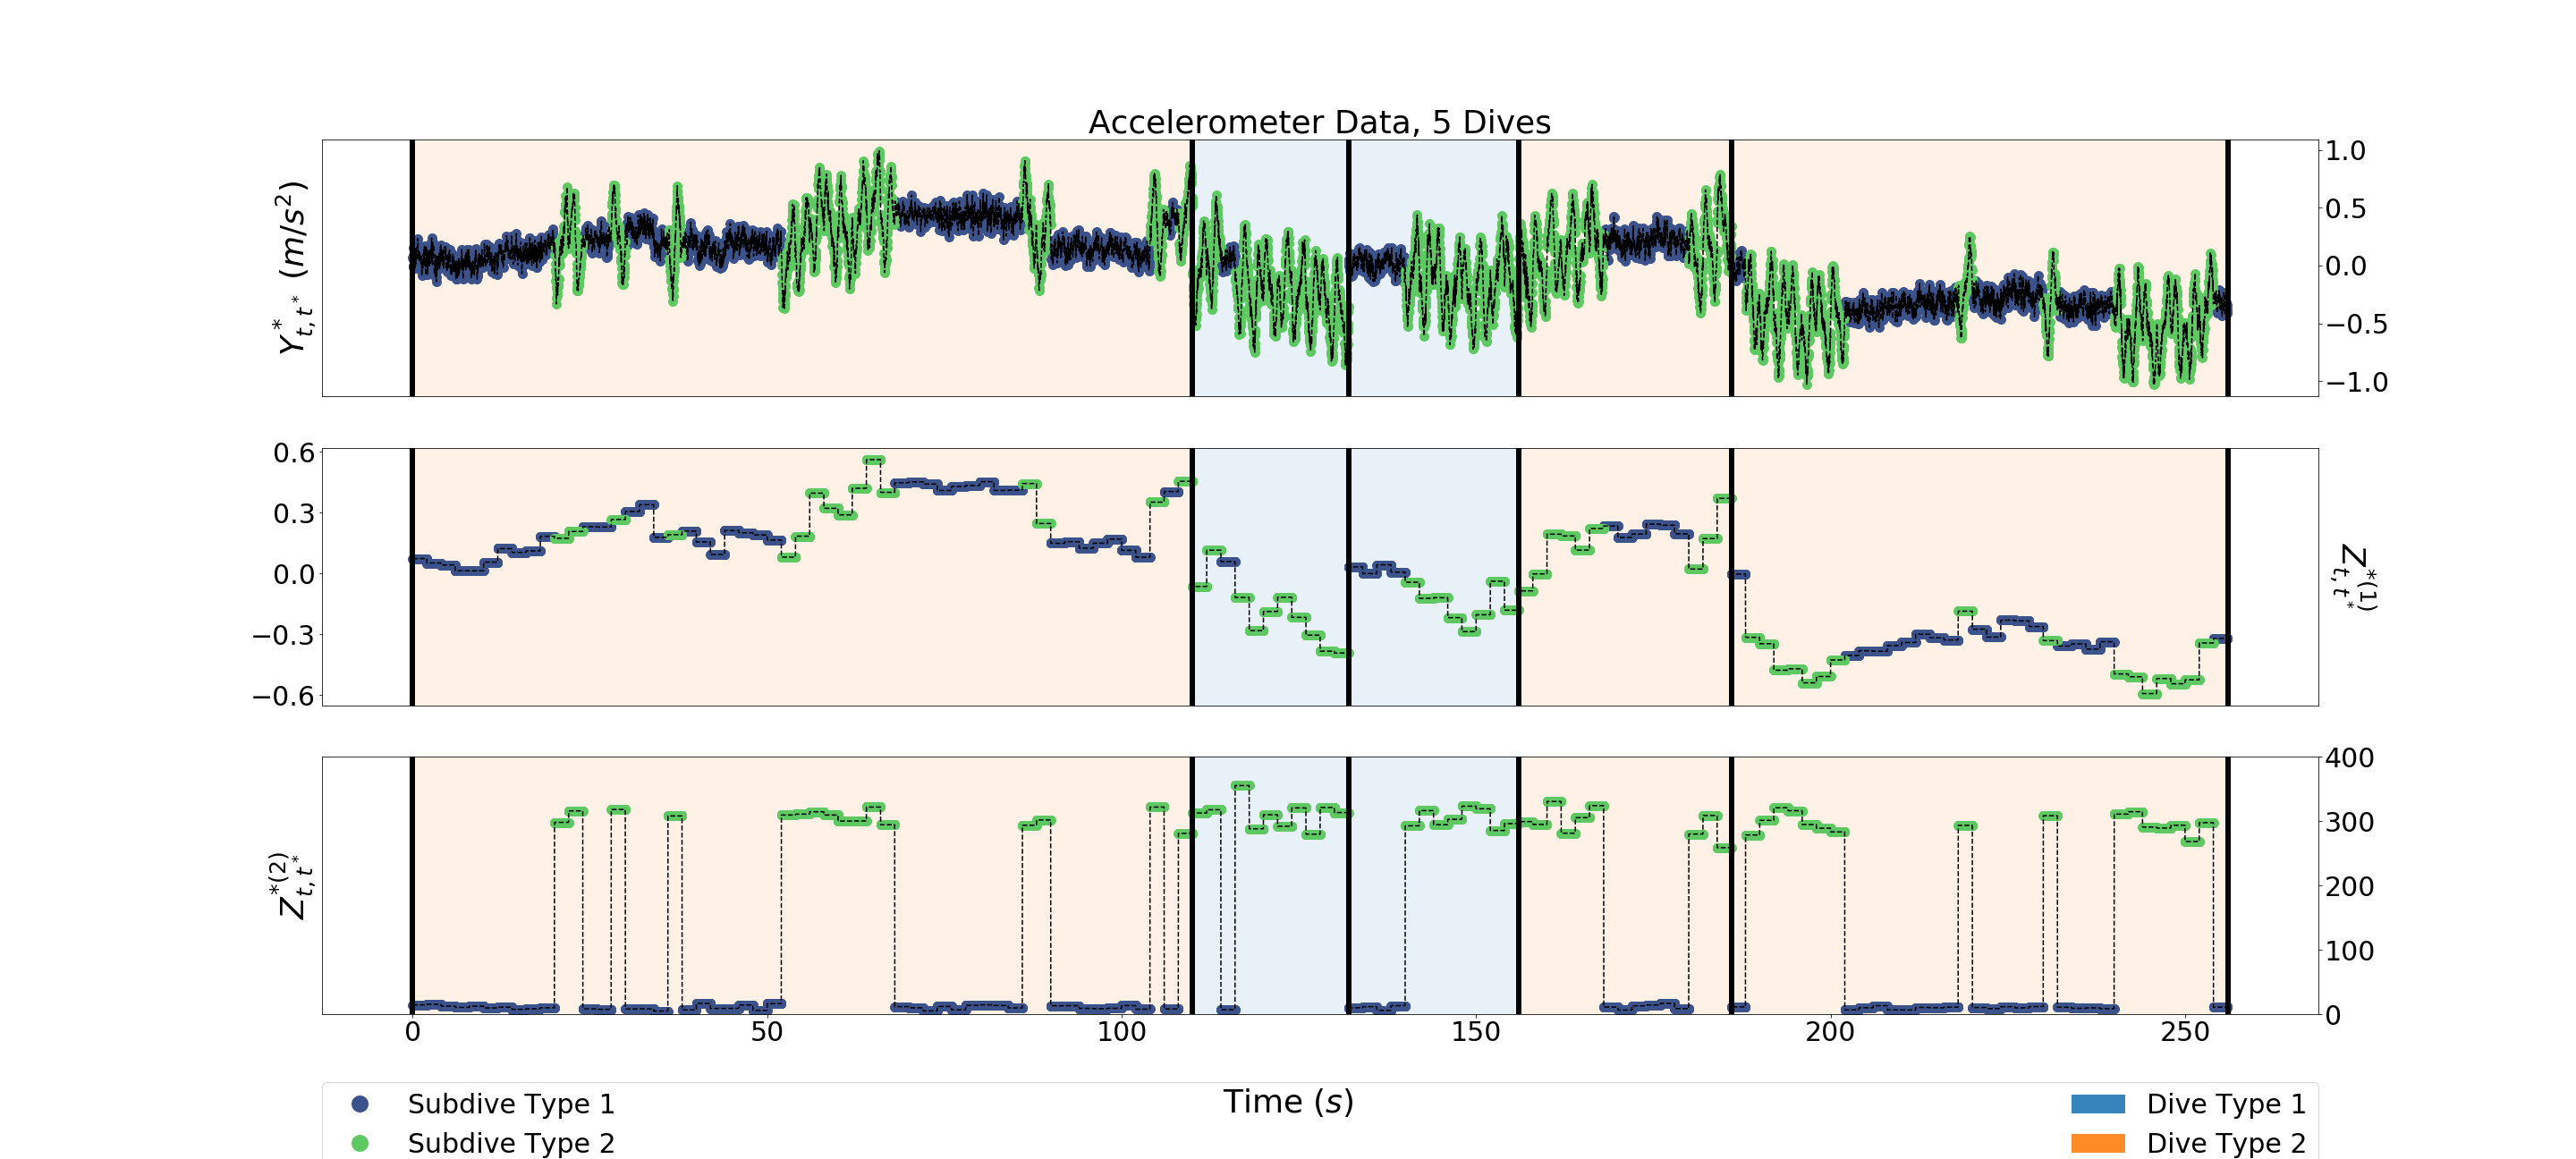
\includegraphics[width=5in]{../Plots/sim_data.png}
	\caption{Acceleration data for one dive of a selected simulated data set. $Y^*$ refers to the raw accelerometer data, and $A^*$ and $W^*$ are kept constant over each two-second window used to train the models. The colour of the line corresponds to the true fine-scale state, while the colour of the background corresponds to the true dive type.}
	\label{fig:sim_data}
\end{figure}

\begin{figure}[ht]
    \centering
    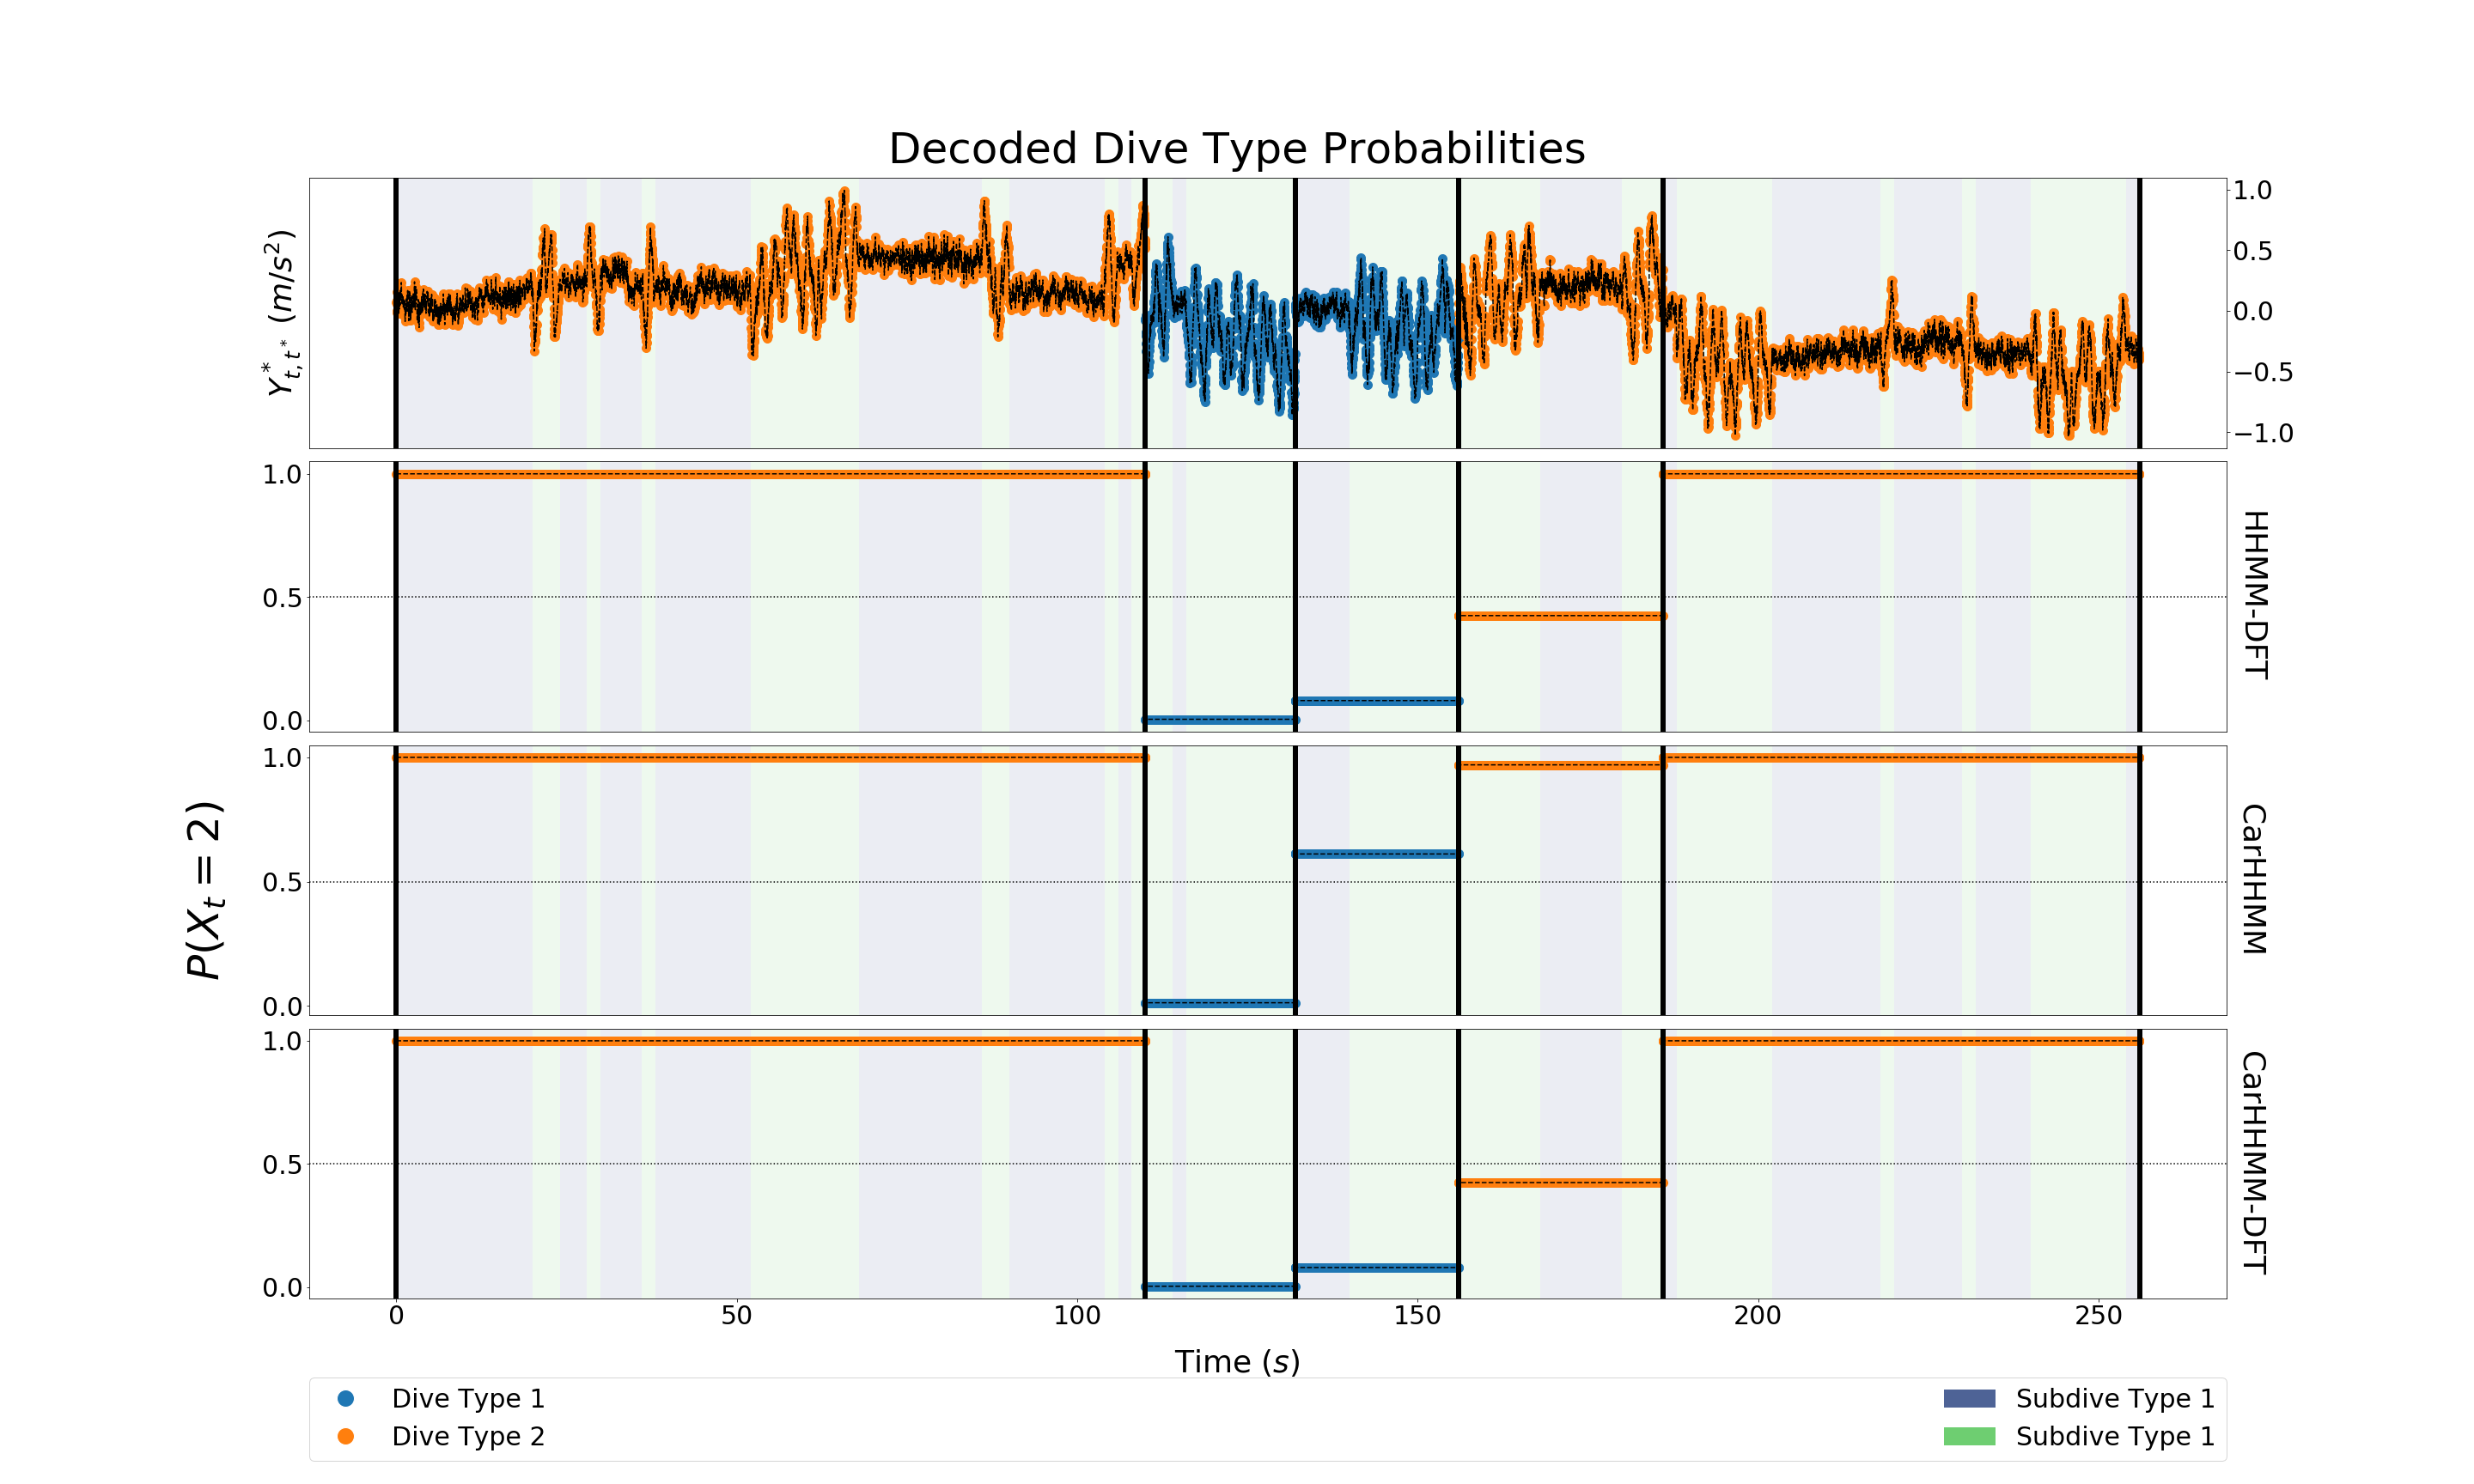
\includegraphics[width=5in]{../Plots/Posterior_Coarse_States.png}
    \caption{Estimated probabilities that each dive is of type two for five selected dives of one simulated data set. The colour of the line corresponds to the true dive type while the colour of the background corresponds to the true subdive state. The CarHMM-DFT is omitted because it assumes there is only one dive type.}
    \label{fig:acc_coarse}
\end{figure}

\begin{figure}[ht]
    \centering
    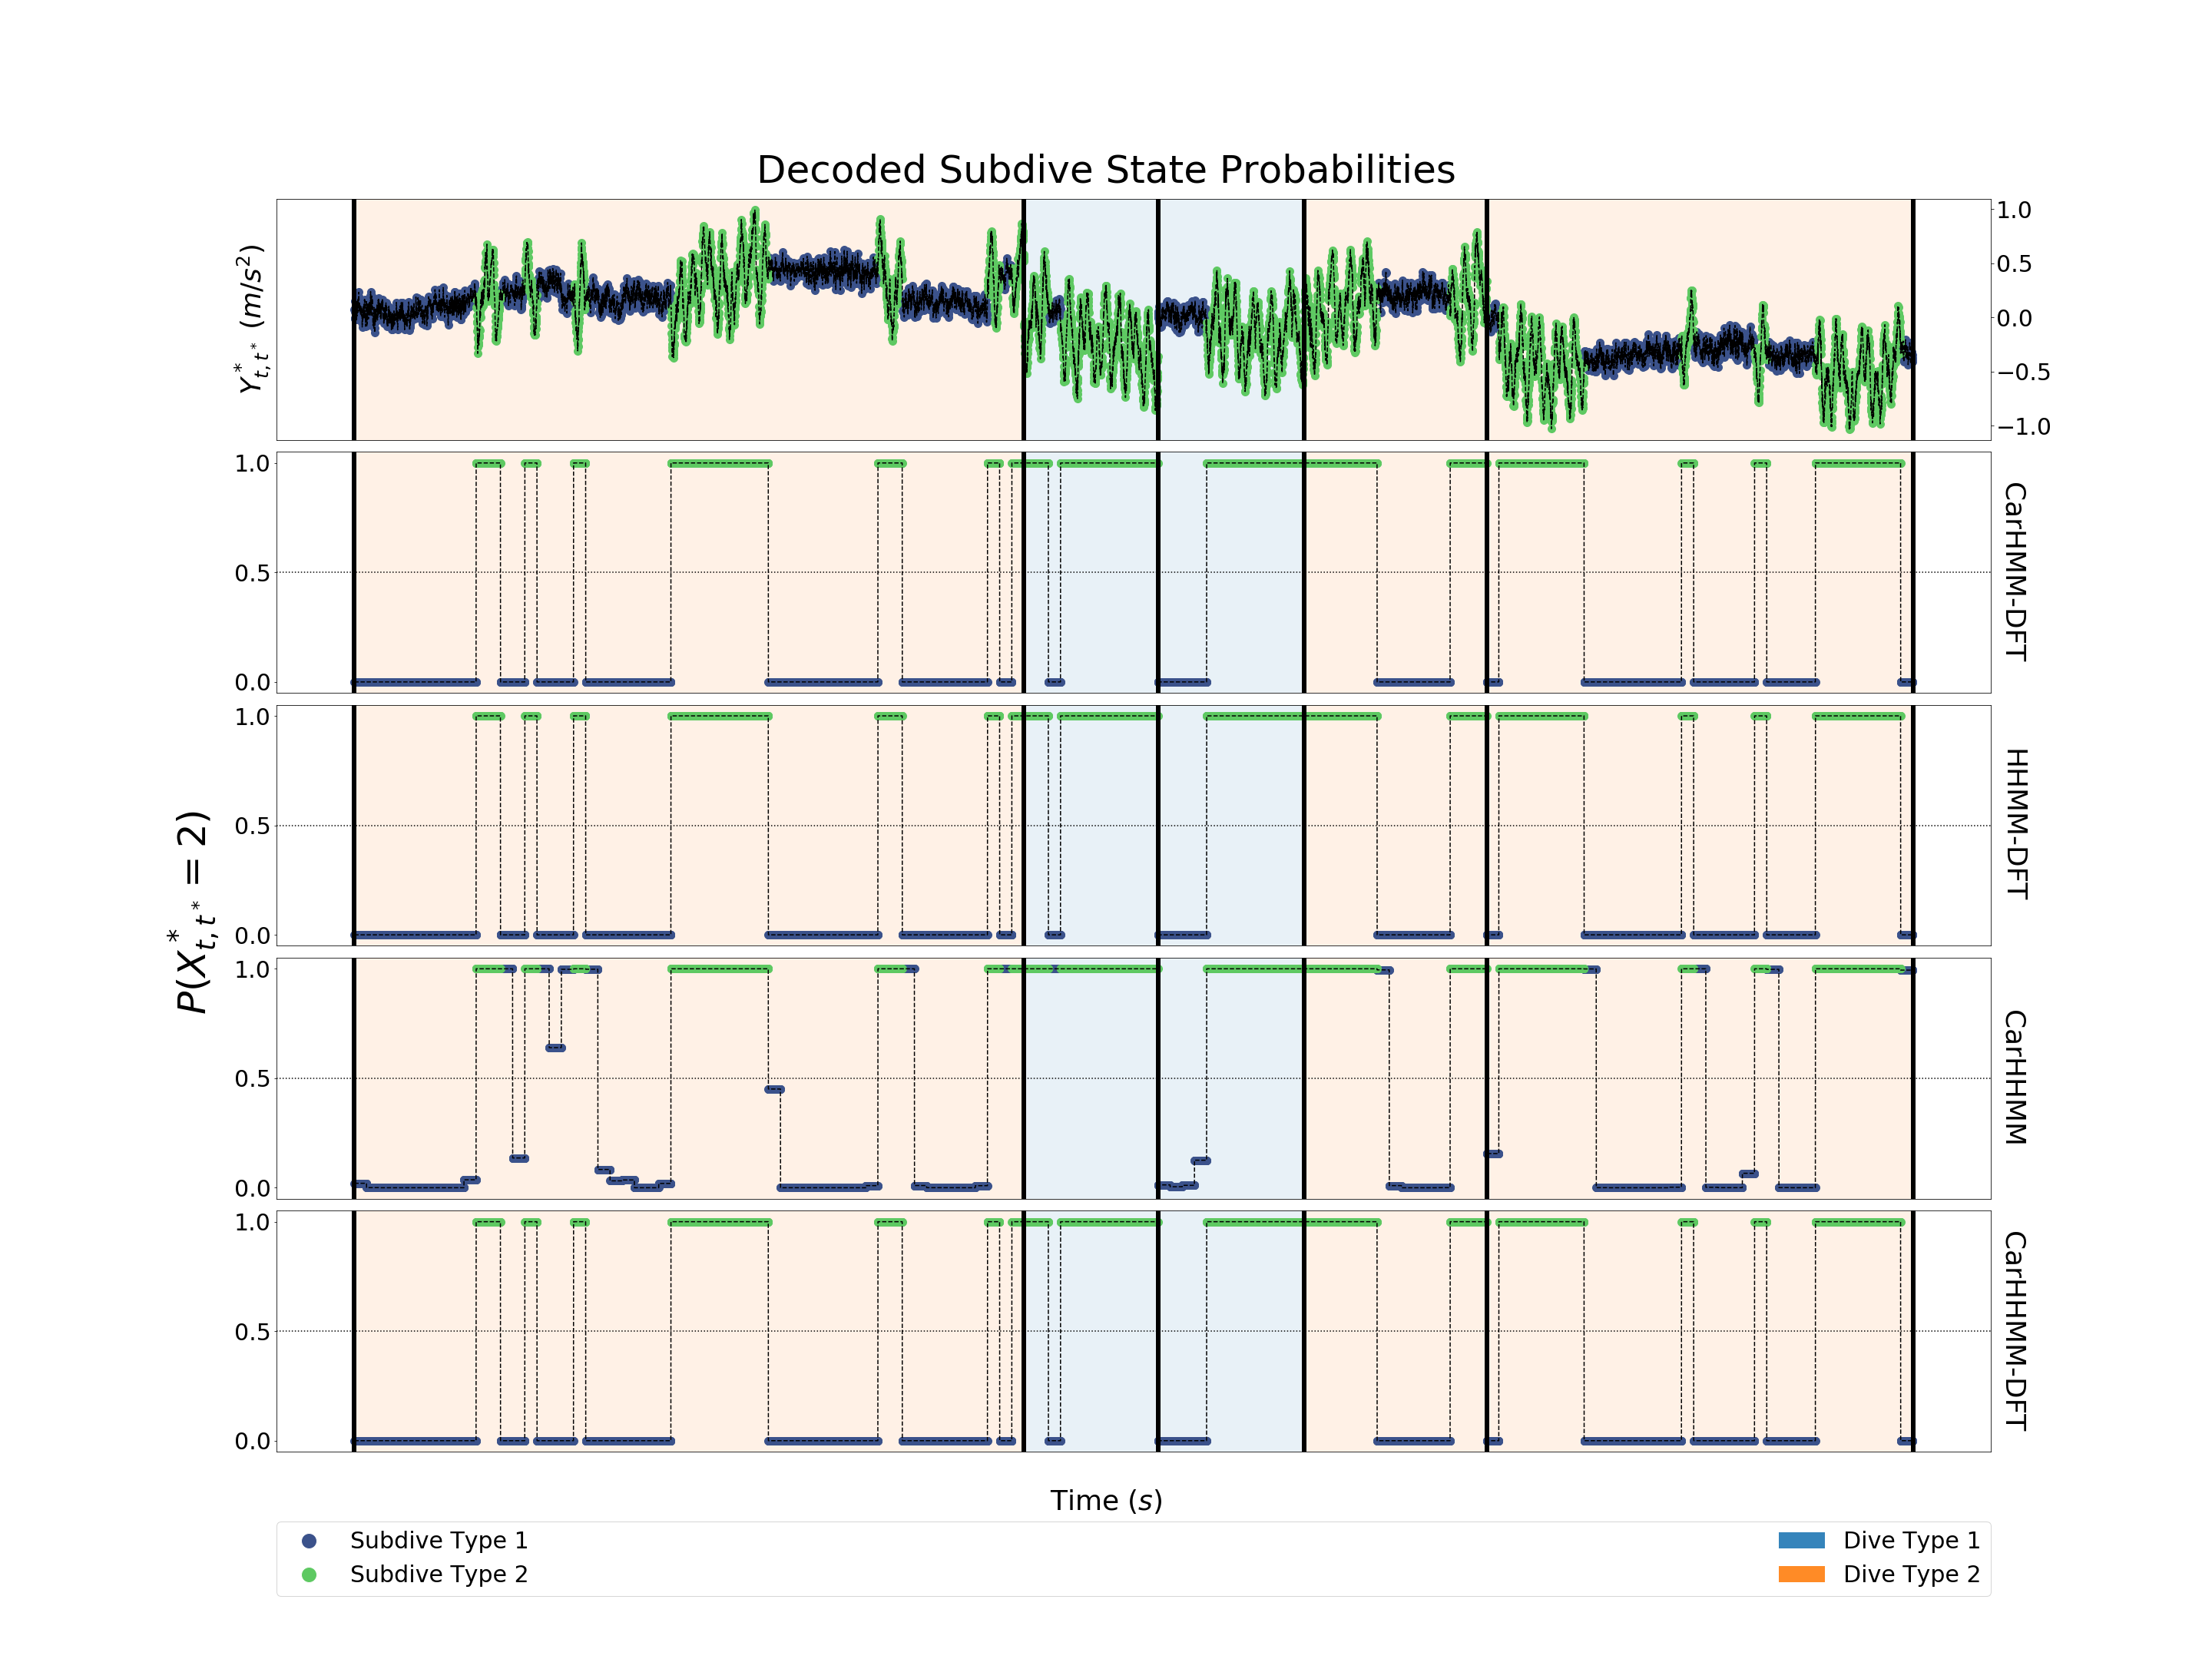
\includegraphics[width=5in]{../Plots/Posterior_Fine_States.png}
    \caption{Estimated probabilities that each subdive segment is in state two for five selected dives of one simulated data set. The colour of the line corresponds to the true subdive state while the colour of the background corresponds to the true dive type.}
    \label{fig:acc_fine}
\end{figure}